\section*{Learning Objectives}
\begin{itemize}
\item How to reduce a hard problem to two much easier problems
\item The concept of ``factoring'' a matrix into a product of two simpler matrices that are in turn useful for solving systems of linear equations. 
\end{itemize}

\section*{Outcomes}
\begin{itemize}
\item Our first encounter in lecture with an explicit algorithm
\item Learn how to do a \textit{special case} of the $LU$ factorization, where $L$ is a lower triangular matrix and $U$ is an upper triangular matrix.

    \item Use the $LU$ factorization to solve linear equations

    \item More advanced: what we missed in our first pass at $LU$ factorization: a (row) permutation matrix.
\end{itemize}
\newpage

\section{Recalling Forward and Back Substitution}

For a lower triangular system of equations with non-zero leading coefficients, such as
\begin{equation}
    \begin{aligned}
     3 x_1 &=6 \\
     2 x_1 - x_2 &= -2\\
    x_1 - 2 x_2 + 3 x_3  &= 2,
    \end{aligned} \iff \left[\begin{array}{rrr} 3 & 0 & 0\\ 2 & -1 & 0 \\   1 & -2 & 3 \end{array} \right] \begin{bmatrix} x_1 \\ x_2 \\ x_3\end{bmatrix} = \left[\begin{array}{r} 6 \\ -2 \\ 2\end{array} \right]
\end{equation}
we can find a solution via forward substitution,
\begin{equation}
    \begin{aligned}
 x_1 &=\frac{1}{3} 6 = 2\\
 x_2 &= -\left[ -2 -2 x_1\right] \\
  x_3  &=\frac{1}{3}\left[ 2 -x_1 + 2 x_2 \right],
    \end{aligned} \implies \left\{ \begin{aligned}
     x_1 &=\frac{1}{3} 6 = 2\\
 x_2 &= 2 + 2 x_1 = 2 + 2(2)=6\\
     x_3  &=\frac{1}{3}\left[ 2 -x_1 + 2 x_2 \right]=\frac{1}{3}\left[ 2 -(2) + 2 (6) \right]=\frac{12}{3} =  4.
    \end{aligned} \right.
\end{equation}


On the other hand, for an upper triangular system of equations with non-zero leading coefficients, such as
\begin{equation}
    \begin{aligned}
     x_1 + 3x_2 + 2 x_3 &=6 \\
     2 x_2 +x_3 &= -2\\
     3 x_3 &= 4,
    \end{aligned} \iff \left[\begin{array}{rrr} 1 & 3 & 2\\ 0 & 2 & 1 \\   0 & 0 & 3 \end{array} \right] \begin{bmatrix} x_1 \\ x_2 \\ x_3\end{bmatrix} = \left[\begin{array}{r} 6 \\ -2 \\ 4\end{array} \right]
\end{equation}
we can find a solution by back substitution,
\begin{equation}
    \begin{aligned}
         x_1  &=6- (3x_2 + 2 x_3) \\
      x_2 &= \frac{1}{2} \left( -2-x_3 \right) \\
      x_3 &= \frac{4}{3},
    \end{aligned} \implies \left\{ 
    \begin{aligned}
         x_1  &=6- (3x_2 + 2 x_3) = 6 -( \frac{3}{3} + \frac{8}{3})=\frac{18}{3}-\frac{11}{3}=2 \frac{1}{3} \\
        x_2 &= \frac{1}{2} \left( -2-x_3 \right) = \frac{1}{2} \left( -2-\frac{4}{3} \right)= \frac{1}{2} \left(\frac{2}{3}\right) = \frac{1}{3}\\
      x_3 &= \frac{4}{3}.
    \end{aligned}  \right.
\end{equation}

\section{Recalling Matrix Multiplication in the Form of Columns Times Rows}

Suppose that $A$ is $n \times k$ and $B$ is $k \times m$ so that the two matrices are compatible for matrix multiplication. Then 
$$A\cdot B = \sum_{i=1}^{k} a_i^{\rm col} \cdot b_i^{\rm row},  $$
the ``sum of the columns of $A$ multiplied by the rows of $B$''.\\

\begin{example}
\label{ex:LUprod}
Form the matrix product of $A=\left[\begin{array}{cc} 1 & 0\\
3 & 4\end{array}\right]$ and $B=\left[\begin{array}{rr}
 5 &2  \\
0 & -1 \end{array}\right].$
\end{example}

\textbf{Solution}

$$A=\left[\begin{array}{cc} 1 & 0\\
3 & 4\end{array}\right] = \left[\begin{array}{cc} a_1^{\rm col} & a_2^{\rm col} \end{array}\right]  = 
\left[ \boxed{\begin{array}{c} 1 \\ 3 \end{array} }~~~
\boxed{\begin{array}{c} 0 \\ 4 \end{array} }\right]
~~\text{and}~~B=\left[\begin{array}{rr}
 5 &2  \\
0 & -1 \end{array}\right] = \left[\begin{array}{c} b_1^{\rm row} \medskip \\
b_2^{\rm row} \end{array}\right]  = \left[\begin{array}{c}\boxed{ 5 ~~~~ 2} \medskip \\
\boxed{ 0 ~~{-1}}
\end{array} \right]$$

$$
a_1^{\rm col}  b_1^{\rm row}= \left[\begin{array}{c} 1 \\
3  \end{array}\right] \cdot \left[\begin{array}{cc}5 & 2 \end{array}\right] = \left[\begin{array}{rr} 5 & 2\\
15 & 6 \end{array}\right]$$
%
$$
a_2^{\rm col}  b_2^{\rm row}= \left[\begin{array}{c} 0\\
4 \end{array}\right] \cdot \left[\begin{array}{rr}0 & -1 \end{array}\right] = \left[\begin{array}{rr} 0 & 0\\
0 & -4 \end{array}\right]$$
and the matrix product is
%
$$A\cdot B=a_1^{\rm col}  b_1^{\rm row} + a_2^{\rm col}  b_2^{\rm row} = \left[\begin{array}{rr} 5 & 2\\
15 & 6 \end{array}\right] + \left[\begin{array}{rr} 0 & 0\\
0 & -4 \end{array}\right]=\left[\begin{array}{rr} 5 & 2\\
15 & 2 \end{array}\right]$$

\Qed



\section{LU (Lower-Upper) Factorization (without row permutations)}
\label{sec:LUwithoutPermutations}

\textbf{As a lead in to our main topic}, note that in Example~\ref{ex:LUprod}, $A$ is a lower triangular matrix, $B$ is an upper triangular matrix, while their product $A\cdot B$ is neither. Can this process be reversed? That is, given a generic square matrix, can we factor it as the product of a lower-triangular matrix and an upper-triangular matrix? And even if we can do such a factorization, would it be helpful?\\

We'll delay an explicit answer to the question of utility because you have a sense already that triangular matrices make your life easier! Let's consider the factorization question for
$$M=\left[\begin{array}{rrr} 
    1   &  4   &  5 \\
     2  &   9  &  17 \\
     3  &  18  &  58 \end{array}  \right]. $$
We define $C_1$  and $R_1$  to be the first column of $M$ and the first row of $M$, respectively, that is
$$C_1=\left[\begin{array}{r} 
    1  \\ 2 \\ 3  \end{array}  \right]~~\text{and}~~R_1=\left[\begin{array}{rrr} 
    1   &  4   &  5 \end{array}  \right].  $$
Then
\begin{align*} 
M - C_1 \cdot R_1 &= \left[\begin{array}{rrr} 
    1   &  4   &  5 \\
     2  &   9  &  17 \\
     3  &  18  &  58 \end{array}  \right] -  \left[\begin{array}{r} 
    1  \\ 2 \\ 3  \end{array}  \right] \cdot \left[\begin{array}{rrr} 
    1   &  4   &  5 \end{array}  \right] \\
    &=  \left[\begin{array}{rrr} 
    1   &  4   &  5 \\
     2  &   9  &  17 \\
     3  &  18  &  58 \end{array}  \right] - 
     \left[\begin{array}{rrr} 
    1   &  4   &  5 \\
     2  &   8  &  10 \\
     3  &  12  &  15 \end{array}  \right]\\
     &=\left[\begin{array}{rrr} 
       0  &   0  &   0 \\
     0   &  1   &  7 \\
     0   &  6   & 43 \end{array}  \right]
\end{align*}

Oh! We have taken a $3 \times 3$ matrix and essentially made it into a $2 \times 2 $ matrix!! Can we do this again? \\

We define $C_2$  and $R_2$  to be the second column and second row of $M- C_1 \cdot R_1$, respectively, that is
$$C_2=\left[\begin{array}{r} 
    0  \\ 1 \\ 6  \end{array}  \right]~~\text{and}~~R_2=\left[\begin{array}{rrr} 
   0   &  1   &  7 \end{array}  \right].  $$
   Then we compute that 
   \begin{align*} 
\left(M - C_1 \cdot R_1 \right)  -  C_2 \cdot R_2 &= \left[\begin{array}{rrr} 
       0  &   0  &   0 \\
     0   &  1   &  7 \\
     0   &  6   & 43 \end{array}  \right] -  \left[\begin{array}{r} 
    0  \\ 1 \\ 6  \end{array}  \right] \cdot \left[\begin{array}{rrr} 
   0   &  1   &  7 \end{array}  \right] \\
     &=\left[\begin{array}{rrr} 
       0  &   0  &   0 \\
     0   &  1   &  7 \\
     0   &  6   & 43 \end{array}  \right] -\left[\begin{array}{rrr} 
       0  &   0  &   0 \\
     0   &  1   &  7 \\
     0   &  6   & 42 \end{array}  \right]\\
     &=\left[\begin{array}{rrr} 
       0  &   0  &   0 \\
     0   &  0   &  0 \\
     0   &  0   & 1 \end{array}  \right]
\end{align*}
     
 Oh! Now we are essentially down to a $1 \times 1 $ matrix!!  We note that if we define  
 $C_3$  and $R_3$  to be the third column and third row of $M- C_1 \cdot R_1 - C_2 \cdot R_2$, respectively, that is
$$C_3=\left[\begin{array}{r} 
    0  \\ 0\\ 1  \end{array}  \right]~~\text{and}~~R_3=\left[\begin{array}{rrr} 
   0   &  0   &  1 \end{array}  \right],  $$
   then 
   $$C_3 \cdot R_3 = \left[\begin{array}{rrr} 
       0  &   0  &   0 \\
     0   &  0   &  0 \\
     0   &  0   & 1 \end{array}  \right],
     $$
     and hence,
     $$M = C_1 \cdot R_1 + C_2 \cdot R_2 + C_3 \cdot R_3 = \left[\begin{array}{rrr} 
   C_1   &  C_2   &  C_3\end{array}  \right] \cdot \left[\begin{array}{r} 
    R_1  \\ R_2\\ R_3 \end{array}  \right]. $$
    
    Moreover, 
    \begin{itemize}
        \item  $L:=\left[\begin{array}{rrr} 
   C_1   &  C_2   &  C_3\end{array}  \right] = 
   \left[\begin{array}{rrr} 
       1  &   0  &   0 \\
    2  &  1   &  0 \\
     3  &  6   & 1 \end{array}  \right]$ is \textbf{lower triangular}, 
     \item $U:=   \left[\begin{array}{r} 
    R_1 \\ R_2\\ R_3  \end{array}  \right] = \left[\begin{array}{rrr} 
     1  &   4   &  5 \\
     0  &   1   &  7 \\
     0  &   0   &  1 \end{array}  \right]$ is \textbf{upper triangular}, and \\
     \item $M=L \cdot U$, the product of a lower triangular matrix and an upper triangular matrix.
    \end{itemize}
    
    \begin{tcolorbox}[title=\textbf{Secret Sauce of LU Factorization}]
    Is that all there is to LU Factorization? No, there's a bit more to it. The real algorithm has a ``normalization step''. To motivate it we take a matrix $M$ that has something other than a one in its $a_{11}$-entry and naively form ``$C_1$'' as the first column of the matrix and ``$R_1$'' as the first row of the matrix. Then 
    $$\underbrace{\left[\begin{array}{rr} 
    2   &  3 \\
4   &  5\end{array}  \right]}_{M} - \underbrace{\left[\begin{array}{r} 
    2\\ 4 \end{array}  \right]}_{\text{``$C_1$''}} \cdot  \underbrace{\left[\begin{array}{rr} 
    2  &   3  \end{array}  \right]}_{\text{``$R_1$''}} =\underbrace{\left[\begin{array}{rr} 
    2   &  3 \\
4   &  5\end{array}  \right]}_{M} - \underbrace{\left[\begin{array}{rr} 
   4  &   6 \\
     8  &  12\end{array}  \right]}_{\text{``$C_1 \cdot R_1$ ''}} = \left[\begin{array}{rr} 
   -2  &   -3 \\
     -4  &  -7\end{array}  \right],  $$
which does NOT result in a matrix with zeros in its leading column and row! However, if we keep $R_1$ as the first row of $M$ but this time, we form $C_1$ from the first column of $M$ normalized by its first entry, then we can make it work. Watch! 
   $$\underbrace{\left[\begin{array}{rr} 
    2   &  3 \\
4   &  5\end{array}  \right]}_{M} - \underbrace{\left[\begin{array}{r} 
    \sfrac{2}{2} \medskip\\ \sfrac{4}{2} \end{array}  \right]}_{C_1} \cdot  \underbrace{\left[\begin{array}{rr} 
    2  &   3  \end{array}  \right]}_{R_1} = \underbrace{\left[\begin{array}{rr} 
    2   &  3 \\
4   &  5\end{array}  \right]}_{M} - \underbrace{\left[\begin{array}{r} 
    1 \medskip\\ 2 \end{array}  \right]}_{C_1} \cdot  \underbrace{\left[\begin{array}{rr} 
    2  &   3  \end{array}  \right]}_{R_1} =\underbrace{\left[\begin{array}{rr} 
    2   &  3 \\
4   &  5\end{array}  \right]}_{M} -\underbrace{\left[\begin{array}{rr} 
    2   &  3 \\
4   &  6\end{array}  \right]}_{C_1 \cdot R_1} = \left[\begin{array}{rr} 
    0   &  0 \\
0  &  -1\end{array}  \right] .  $$


\textcolor{red}{\textbf{Warning:}}  When we do the normalization, we could get into trouble with a divide by zero!
      
    \end{tcolorbox}
    
    
\textbf{More generally,} if we assume that $\mathbf{a_{11}} \neq 0$,
\begin{align*}
     \left[\begin{array}{cccc} \mathbf{a_{11}}& \mathbf{a_{12} }& \cdots & \mathbf{a_{1n}} \medskip \\
\mathbf{ a_{21} }& a_{22}& \cdots & a_{2n}  \\
 \vdots & \vdots&  \ddots & \vdots \\
 \mathbf{a_{n1} }& a_{n2}& \cdots & a_{nn} 
 \end{array}\right]- \left[\begin{array}{c} \mathbf{1.0} \medskip \\
\mathbf{\sfrac{a_{21}}{a_{11}}} \\
 \vdots \\
 \mathbf{\sfrac{a_{n1}}{a_{11}} }
 \end{array}\right] \cdot \left[\begin{array}{cccc} \mathbf{a_{11}} & \mathbf{a_{12}} & \cdots & \mathbf{a_{1n} }
 \end{array}\right]&= \left[\begin{array}{cccc} \mathbf{a_{11}}& \mathbf{a_{12} }& \cdots & \mathbf{a_{1n}} \medskip \\
\mathbf{ a_{21} }& a_{22}& \cdots & a_{2n}  \\
 \vdots & \vdots&  \ddots & \vdots \\
 \mathbf{a_{n1} }& a_{n2}& \cdots & a_{nn} 
 \end{array}\right] - \left[\begin{array}{cccc} \mathbf{a_{11}} & \mathbf{a_{12} } & \cdots & \mathbf{a_{1n}} \\
 &\\
 \mathbf{a_{21} }& \ast & \cdots & \ast \\
 \vdots & \vdots&  \ddots & \vdots \\
 \mathbf{a_{n1} }& \ast& \cdots & \ast 
 \end{array}\right]  \bigskip \\
 &= \left[\begin{array}{cccc} \mathbf{0} & \mathbf{0} & \cdots & \mathbf{0} \medskip \\
\mathbf{0} & \ast & \cdots & \ast \\
 \vdots & \vdots&  \ddots & \vdots \\
\mathbf{0} & \ast& \cdots & \ast 
 \end{array}\right]
 \end{align*}
    
   
\vspace*{.4cm}


\begin{tcolorbox}[sharp corners, colback=green!30, colframe=green!80!blue, title=\textbf{\Large LU Factorization}]
\begin{algorithm}[H]
\SetAlgoLined
\KwResult{For M an $n \times n$ square matrix, with $n\ge2$, find $L$ and $U$ such that $M=LU$}
\mbox{} \\
 \textbf{\# initialization:}\\
 {\rm Temp}=copy(M); \\
L = Array\{Float64,2\}(undef, n, 0)  ~~~\# L=[] Empty matrix\\
U = Array\{Float64,2\}(undef, 0, n)  ~~~\# U=[] Empty matrix\\
  \textbf{\# end initialization:}\\
  \mbox{} \\
\For{k=1:n} 
 {
    \# Julia does NOT place a \textbf{do} as part of a \textbf{for loop} \\
    \# \textbf{for} l=1:n i show it will look in Julia\\
    C=Temp[:,k]; \# k-th column \\
        pivot=C[k]; \\
    R={\rm Temp}[k,:]'; \# k-th row, which in Julia, requires a transpose\\
    \# Alternative R={\rm Temp}[k:k,:] ~\# also works in Julia for k-th row\\
  \eIf{ ! isapprox(pivot, 0, atol = 1E-8) \# check for zero} 
  { 
    \# Julia does not place a \textbf{then} as part of an  \textbf{if statement}\\
    \# \textbf{if} ! isapprox(pivot, 0, atol = 1E-8) is how it will look in Julia
    C=C/pivot; \# normalize so that $k$-th entry is equal to 1.0 \\
    {\rm Temp}={\rm Temp}-C*R; \\
     L=[L C];  \# Build the lower-triangular matrix by columns\\
    U=[U;R]; \# Build the upper-triangular matrix by rows\;
   }
   {
   println(``Matrix requires row permutations'') \\
   println(``Step where algorithm failed is k= \$k'')   \\
   break~~~\# Jump out of the for loop and terminate the algorithm 
  }
}
\mbox{ } \\
   \textbf{return L, U}
 \caption{LU-Factorization (without permutations)}
\end{algorithm}
\end{tcolorbox}

The algorithm is easy to do by hand for very small matrices. In Julia, you can write code that will do the $LU$ factorization of a $1000 \times 1000$ matrix in a few seconds. The \texttt{lu} function in the LinearAlgebra package of Julia can do it in a few milliseconds! The exact command is\\

\begin{lstlisting}[language=Julia]
  using LinearAlgebra
  L, U = lu(M, Val(false))
\end{lstlisting}
to return $L$ and $U$ \textbf{without permutations}. If you leave off `` \texttt{Val(false)}'', then the algorithm uses row permutations and you should call it as 
\begin{lstlisting}[language=Julia]
  using LinearAlgebra
  F = lu(M)
  L=F.L
  U=F.U
  P=F.P
\end{lstlisting} 
\vspace*{0.2cm}

\begin{example}
\label{ex:Lu01} 
\textbf{(${\bf 2 \times 2}$ Matrix)} Perform the LU Factorization of $M=\left[\begin{array}{rr} 5 & 2\\
15 & 2 \end{array}\right]$, a $2 \times 2$ square matrix.
\end{example}

\textbf{Solution:}  We'll do every step, just as you would program it up.\\

We \textit{initialize} our algorithm by $${\rm Temp}:= M = \left[\begin{array}{rr} 5 & 2\\
15 & 2 \end{array}\right], L:=[\textrm{empty matrix}],~\text{and}~~ U:=[\textrm{empty matrix}]$$

$\textbf{k=1:}$ We start with $C$ as the first column of ${\rm Temp}$ scaled by the $k=1$ entry of $C$, and thus\footnote{In HW solutions or exams, it is fine to skip a step and write down $L$ directly, however, it is then more difficult to give you a lot of partial credit.}
\begin{align*}C &= \left[\begin{array}{r} 5 \\ 15 \end{array} \right]\\
\textrm{pivot}&=C[1] = 5\\
C&=C. \slash \textrm{pivot} \\
&= \left[\begin{array}{r} 5 \\ 15 \end{array} \right] \cdot \frac{1}{5}\\ 
&= \left[\begin{array}{r} 1 \\ 3\end{array} \right], \end{align*}
while $R$ is the first row of  ${\rm Temp}$ 
$$ R = \left[\begin{array}{rr} 5 & 2 \end{array} \right].$$
We finish up the first step by defining
\begin{align*}
    {\rm Temp}:=& {\rm Temp}-C \cdot R \\
    =& \left[\begin{array}{rr} 5 & 2\\
15 & 2 \end{array}\right] -  \left[\begin{array}{r} 1 \\ 3 \end{array} \right] \cdot  \left[\begin{array}{rr} 5 & 2 \end{array} \right] \\
=&  \left[\begin{array}{rr} 5 & 2\\
15 & 2 \end{array}\right] -   \left[\begin{array}{rr} 5 & 2\\
15 & 6 \end{array}\right] \\
=&   \left[\begin{array}{rr} 0 & 0\\
0 & -4\end{array}\right] \\
\\
L=&[L,C] = \left[\begin{array}{r} 1 \\ 3\end{array} \right]\\
U=&[U;R] = \left[\begin{array}{rr} 5 & 2 \end{array} \right]
\end{align*}

\begin{tcolorbox}[sharp corners, colback=green!30, colframe=green!80!blue, title=\textbf{\large Why LU Factorization Works}]
We observe that $L$ and $U$ were defined so that their product exactly matched the first column and row of $M$. Hence, when we subtract them from $M$, we are left with a problem that is effectively one dimension lower, meaning, in this case, the non-zero part is $1 \times 1$. 
\end{tcolorbox}
While you may be able to finish the factorization by ``inspection'', we will do the complete algorithm just like you would do in a program.\\

$\textbf{k=2:}$ $C$ is the second column of ${\rm Temp}$ scaled by its $k=2$ entry,
\begin{align*}C&=\left[\begin{array}{r} 0\\  -4 \end{array} \right]\\
\textrm{pivot}&=C[2] = -4\\
C&=\left[\begin{array}{r} 0\\  -4 \end{array} \right].\slash \textrm{pivot} \\
&= \left[\begin{array}{r} 0\\  -4 \end{array} \right] \cdot \frac{-1}{4}\\
&= \left[\begin{array}{r} 0\\  1 \end{array} \right], 
\end{align*}
while $R$ is the second row of ${\rm Temp}$,
$$ R = \left[\begin{array}{rr} 0 & -4 \end{array} \right].$$

\begin{align*}
    {\rm Temp}:=& {\rm Temp}-C \cdot R \\
    =& \left[\begin{array}{rr} 0 & 0\\
0 & -4 \end{array}\right] -  \left[\begin{array}{r} 0 \\ 1 \end{array} \right] \cdot  \left[\begin{array}{rr} 0 & -4 \end{array} \right] \\
=&  \left[\begin{array}{rr} 0 & 0\\
0 & -4 \end{array}\right] -   \left[\begin{array}{rr} 0 & 0\\
0 & -4 \end{array}\right] \\
=&   \left[\begin{array}{rr} 0 & 0\\
0 & 0\end{array}\right] \\
\\
L=&[L,C] = \left[\begin{array}{rr} 1 & 0\\ 3 & 1\end{array} \right] = ~\textrm{lower triangular matrix}\\
U=&[U;R] = \left[\begin{array}{rr} 5 & 2 \\ 0 & -4\end{array} \right] = ~\textrm{upper triangular matrix}
\end{align*}

\begin{tcolorbox}[title = \textbf{\large Let's remind ourselves why this works:} ]
The matrix product $L \cdot U$ is equal to the sum of the columns of $L$ times the rows of $U$. The columns and rows were iteratively designed to remove columns and rows from $M$. Indeed, 
\begin{align*}
    {\rm Temp}:=& M-L \cdot U \\
    =& \left[\begin{array}{rr} 5 & 2\\
15 & 2 \end{array}\right] -   \left[\begin{array}{rr} 1 & 0\\ 3& 1 \end{array} \right] \cdot \left[\begin{array}{rr} 5 &  2\\ 0 & -4 \end{array} \right] \\
=& \left[\begin{array}{rr} 5 & 2\\
15 & 2 \end{array}\right] - \left(  \left[\begin{array}{r} 1\\ 3 \end{array} \right] \cdot \left[\begin{array}{rr} 5 &  2 \end{array} \right] + \left[\begin{array}{r}  0\\  1 \end{array} \right] \cdot \left[\begin{array}{rr}  0 & -4 \end{array} \right]  \right) \\
=&  \left[\begin{array}{rr} 5 & 2\\
15 & 2 \end{array}\right] -    \left( \left[\begin{array}{rr} 5 & 2\\
15 & 6 \end{array}\right] +  \left[\begin{array}{rr} 0 & 0\\
0 & -4\end{array}\right]\right) \\ %%
=&  \left[\begin{array}{rr} 5 & 2\\
15 & 2 \end{array}\right] -    \left[\begin{array}{rr} 5 & 2\\
15 & 6 \end{array}\right] -  \left[\begin{array}{rr} 0 & 0\\
0 & -4\end{array}\right] \\ %%
=& \left( \left[\begin{array}{rr} 5 & 2\\
15 & 2 \end{array}\right] -    \left[\begin{array}{rr} 5 & 2\\
15 & 6 \end{array}\right] \right)-  \left[\begin{array}{rr} 0 & 0\\
0 & -4\end{array}\right] \\ %%
 =& \left(  \left[\begin{array}{rr} 0 & 0\\
0 & -4\end{array}\right] \right)-  \left[\begin{array}{rr} 0 & 0\\
0 & -4\end{array}\right] \\ %%
=&   \left[\begin{array}{rr} 0 & 0\\
0 & 0\end{array}\right]
\end{align*}
\end{tcolorbox}
\vspace*{0.2cm}
Hence,
$$
\underbrace{\left[\begin{array}{rr} 5 & 2\\
15 & 2 \end{array}\right]}_{M} =  \underbrace{\left[\begin{array}{rr} 1 & 0\\ 3& 1 \end{array} \right]}_{L} \cdot \underbrace{ \left[\begin{array}{rr} 5 &  2\\ 0 & -4 \end{array} \right] }_{U} $$
\Qed

\vspace*{1cm}
\begin{example}
\label{ex:Lu02} 
\textbf{(${\bf 3 \times 3}$ Matrix)} Perform the LU Factorization of $M=\left[\begin{array}{rrr} -2 & -4 & -6\\
-2 & 1 & -4 \\ -2 & 11 & -4 \end{array}\right]$, a $3 \times 3$ square matrix. 
\end{example}

\textbf{Solution:} We \textit{initialize} our algorithm by $${\rm Temp}:= M = \left[\begin{array}{rrr} -2 & -4 & -6\\
-2 & 1 & -4 \\ -2 & 11 & -4 \end{array}\right], L:=[\textrm{empty matrix}],~\text{and}~~ U:=[\textrm{empty matrix}]$$


$\textbf{k=1:}$ We start with $C$ as first column of ${\rm Temp}$ normalized by $C[1]$ so that its first entry is one
\begin{align*}C &=\left[\begin{array}{r} -2 \\ -2 \\ -2 \end{array} \right]\\
\textrm{pivot}&=C[1] = -2\\
C&=C. \slash \textrm{pivot} \\
&= \left[\begin{array}{r} 1 \\ 1 \\1 \end{array} \right],
\end{align*}
while $R$ is the first row of  ${\rm Temp}$ 
$$ R = \left[\begin{array}{rrr} -2&-4 & -6 \end{array} \right].$$
We finish up the first step by defining
\begin{align*}
    {\rm Temp}:=& {\rm Temp}-C \cdot R \\
    =& \left[\begin{array}{rrr} -2 & -4 & -6\\
-2 & 1 & -4 \\ -2 & 11 & -4 \end{array}\right] -   \left[\begin{array}{r} 1 \\ 1 \\1 \end{array} \right] \cdot  \left[\begin{array}{rrr} -2&-4 & -6 \end{array} \right] \\
=& \left[\begin{array}{rrr} -2 & -4 & -6\\
-2 & 1 & -4 \\ -2 & 11 & -4 \end{array}\right] -   \left[\begin{array}{rrr}  -2&-4 & -6 \\  -2&-4 & -6 \\  -2&-4 & -6\end{array} \right]  \\
=&  \left[\begin{array}{rrr} 0 & 0 & 0\\
0 & 5 & 2 \\ 0 & 15 & 2\end{array}\right]\\
\\
L=&[L,C] = \left[\begin{array}{r}  1 \\ 1 \\1 \end{array} \right]\\
U=&[U;R] = \left[\begin{array}{rrr}  -2&-4 & -6  \end{array} \right]
\end{align*}

\begin{tcolorbox}[sharp corners, colback=green!30, colframe=green!80!blue, title=\textbf{\large Reminder of Why LU Factorization Works}]
We observe that $L$ and $U$ have been constructed so that their product exactly matches the first column and first row of $M$.  Hence, when we subtract $L \cdot U$ from $M$, we are left with a problem that is effectively one dimension lower, meaning, in this case, the non-zero part is $2 \times 2$. 
\end{tcolorbox}
Your wily instructor has arranged for the $2 \times 2$ matrix that remains to be an example that we have already worked! Nevertheless, we will complete the algorithmic steps just like you would do in Julia.\\

$\textbf{k=2:}$ C is the second column of ${\rm Temp}$ scaled by its $ k=2$ entry,
\begin{align*}
    C &= \left[ \begin{array}{r} 0 \\ 5 \\15 \end{array} \right] \\
    \textrm{pivot} &= C[2] = 5 \\
    C &= \left[ \begin{array}{r} 0\\ 5 \\ 15 \end{array} \right] .\slash \textrm{pivot} \\
    &= \left[ \begin{array}{r} 0 \\ 5 \\ 15 \end{array} \right] \cdot \frac{1}{5} \\
    &= \left[ \begin{array}{r} 0 \\ 1 \\ 3 \end{array} \right],
\end{align*}

while R is the second row of ${\rm Temp}$,
$$ R = \left[ \begin{array}{rrr} 0 & 5 & 2 \end{array} \right]. $$

\begin{align*}
    {\rm Temp} :=& {\rm Temp} - C \cdot R \\
    =& \left[ \begin{array}{rrr} 0 & 0 & 0 \\ 0 & 5 & 2 \\ 0 & 15 & 2 \end{array} \right]
    - \left[ \begin{array}{r} 0 \\ 1 \\ 3 \end{array} \right] \cdot \left[ \begin{array}{rrr} 0 & 5 & 2 \end{array} \right] \\
    =& \left[ \begin{array}{rrr} 0 & 0 & 0 \\ 0 & 5 & 2 \\ 0 & 15 & 2 \end{array} \right] - \left[ \begin{array}{rrr} 0 & 0 & 0 \\ 0 & 5 & 2 \\ 0 & 15 & 6 \end{array} \right] \\
    =& \left[ \begin{array}{rrr} 0 & 0 & 0 \\ 0 & 0 & 0 \\ 0 & 0 & -4 \end{array} \right] \\
    \\
    L =& [L, C] = \left[ \begin{array}{rr} 1 & 0 \\ 1 & 1 \\ 1 & 3 \end{array} \right] \\
    U =& [U; R] = \left[ \begin{array}{rrr} -2 & -4 & -6 \\ 0 & 5 & 2 \end{array}\right]
\end{align*}

\begin{tcolorbox}[sharp corners, colback=green!30, colframe=green!80!blue, title = \textbf{Another Reminder:} ]
We observe that $L$ and $U$ have been constructed so that their product exactly matches the first two columns and first two rows of $M$. Hence, when we subtract $L \cdot U$ from $M$, we are left with a problem that is effectively two dimensions lower, meaning, in this case, the non-zero part is $1 \times 1$. 
\end{tcolorbox}
As before, we do the complete algorithm just like you would do in Julia.\\

$\textbf{k=3:}$ C is the third column of ${\rm Temp}$ scaled by its $k=3$ entry,
\begin{align*}
    C &= \left[ \begin{array}{r} 0 \\ 0 \\ -4 \end{array} \right] \\
    \textrm{pivot} &= C[3] = -4 \\
    C &= \left[ \begin{array}{r} 0 \\ 0 \\ -4 \end{array} \right] .\slash \textrm{pivot} \\
    &= \left[ \begin{array}{r} 0 \\ 0 \\ -4 \end{array} \right] \cdot \frac{1}{-4} \\ 
    &= \left[ \begin{array}{r} 0 \\ 0 \\ 1 \end{array} \right],
\end{align*}
while $R$ is the third row of $\rm Temp$,
$$ R = \left[ \begin{array}{rrr} 0 & 0 & -4 \end{array} \right]. $$

\begin{align*}
    {\rm Temp} :=& {\rm Temp} - C \cdot R \\
    =& \left[ \begin{array}{rrr} 0 & 0 & 0 \\ 0 & 0 & 0 \\ 0 & 0 & -4 \end{array} \right] 
    - \left[ \begin{array}{r} 0 \\ 0 \\ 1 \end{array} \right] \cdot \left[ \begin{array}{rrr} 0 & 0 & -4 \end{array} \right] \\
    =& \left[ \begin{array}{rrr} 0 & 0 & 0 \\ 0 & 0 & 0 \\ 0 & 0 & -4 \end{array} \right] - \left[ \begin{array}{rrr} 0 & 0 & 0 \\ 0 & 0 & 0 \\ 0 & 0 & -4 \end{array} \right] \\
    =& \left[ \begin{array}{rrr} 0 & 0 & 0 \\ 0 & 0 & 0 \\ 0 & 0 & 0 \end{array} \right] \\
    \\
    L =& [L, C] = \left[ \begin{array}{rrr} 1 & 0 & 0 \\ 1 & 1 & 0 \\ 1 & 3 & 1 \end{array} \right] = ~\textrm{lower triangular matrix} \\
    U =& [U; R] = \left[ \begin{array}{rrr} -2 & -4 & -6 \\ 0 & 5 & 2 \\ 0 & 0 & -4 \end{array} \right] = ~\textrm{upper triangular matrix}
\end{align*}

\begin{tcolorbox}[title=\textbf{\Large Let's remind ourselves why this works:}]
 As before,
\begin{align*}
    {\rm Temp} :=& M - L \cdot U \\
    =& \left[ \begin{array}{rrr} -2 & -4 & -6 \\ -2 & 1 & -4 \\ -2 & 11 & -4 \end{array} \right] 
    - \left[ \begin{array}{rrr} 1 & 0 & 0 \\ 1 & 1 & 0 \\ 1 & 3 & 1 \end{array} \right] \cdot \left[ \begin{array}{rrr} -2 & -4 & -6 \\ 0 & 5 & 2 \\ 0 & 0 & -4 \end{array} \right] \\
    =& \left[ \begin{array}{rrr} -2 & -4 & -6 \\ -2 & 1 & -4 \\ -2 & 11 & -4 \end{array} \right]
    - \left( \left[ \begin{array}{r} 1 \\ 1 \\ 1 \end{array} \right] \cdot \left[ \begin{array}{rrr} -2 & -4 & -6 \end{array} \right] + \left[ \begin{array}{r} 0 \\ 1 \\ 3 \end{array} \right] \cdot \left[ \begin{array}{rrr} 0 & 5 & 2 \end{array} \right] + \left[ \begin{array}{r} 0 \\ 0 \\ 1 \end{array} \right] \cdot \left[ \begin{array}{rrr} 0 & 0 & -4 \end{array} \right] \right) \\
    =& \left[ \begin{array}{rrr} -2 & -4 & -6 \\ -2 & 1 & -4 \\ -2 & 11 & -4 \end{array} \right] 
    - \left( \left[ \begin{array}{rrr} -2 & -4 & -6 \\ -2 & -4 & -6 \\ -2 & -4 & -6 \end{array} \right] +  \left[ \begin{array}{rrr} 0 & 0 & 0 \\ 0 & 5 & 2 \\ 0 & 15 & 6 \end{array} \right] + \left[ \begin{array}{rrr} 0 & 0 & 0 \\ 0 & 0 & 0 \\ 0 & 0 & -4 \end{array} \right] \right) \\ 
    =& \left[ \begin{array}{rrr} -2 & -4 & -6 \\ -2 & 1 & -4 \\ -2 & 11 & -4 \end{array} \right] 
    - \left[ \begin{array}{rrr} -2 & -4 & -6 \\ -2 & -4 & -6 \\ -2 & -4 & -6 \end{array} \right] -  \left[ \begin{array}{rrr} 0 & 0 & 0 \\ 0 & 5 & 2 \\ 0 & 15 & 6 \end{array} \right] - \left[ \begin{array}{rrr} 0 & 0 & 0 \\ 0 & 0 & 0 \\ 0 & 0 & -4 \end{array} \right] \\ 
    =& \left( \left[ \begin{array}{rrr} -2 & -4 & -6 \\ -2 & 1 & -4 \\ -2 & 11 & -4 \end{array} \right] - \left[ \begin{array}{rrr} -2 & -4 & -6 \\ -2 & -4 & -6 \\ -2 & -4 & -6 \end{array} \right] \right) -  \left[ \begin{array}{rrr} 0 & 0 & 0 \\ 0 & 5 & 2 \\ 0 & 15 & 6 \end{array} \right] - \left[ \begin{array}{rrr} 0 & 0 & 0 \\ 0 & 0 & 0 \\ 0 & 0 & -4 \end{array} \right] \\ 
    =& \left( \left[ \begin{array}{rrr} 0 & 0 & 0 \\ 0 & 5 & 2 \\ 0 & 15 & 2 \end{array} \right] -  \left[ \begin{array}{rrr} 0 & 0 & 0 \\ 0 & 5 & 2 \\ 0 & 15 & 6 \end{array} \right] \right) - \left[ \begin{array}{rrr} 0 & 0 & 0 \\ 0 & 0 & 0 \\ 0 & 0 & -4 \end{array} \right] \\ 
    =& \left[ \begin{array}{rrr} 0 & 0 & 0 \\ 0 & 0 & 0 \\ 0 & 0 & -4 \end{array} \right] - \left[ \begin{array}{rrr} 0 & 0 & 0 \\ 0 & 0 & 0 \\ 0 & 0 & -4 \end{array} \right] \\ 
    =& \left[ \begin{array}{rrr} 0 & 0 & 0 \\ 0 & 0 & 0 \\ 0 & 0 & 0 \end{array} \right] \\ 
\end{align*}
\end{tcolorbox}

Hence,

$$\underbrace{\left[\begin{array}{rrr} -2 & -4 & -6\\
-2 & 1 & -4 \\ -2 & 11 & -4 \end{array}\right]}_{M} =  \underbrace{\left[\begin{array}{rrr} 1 & 0 & 0\\ 1 & 1 & 0\\ 1 & 3  & 1\end{array} \right]}_{L} \cdot \underbrace{\left[\begin{array}{rrr} -2 & -4 & -6 \\ 0 & 5 &  2 \\ 0 &  0 & -4\end{array} \right]}_{U} $$

\Qed

\section{LU Factorization for Solving Linear Equations}
\label{sec:LUsolveAxEqB}

\begin{tcolorbox}[title=\Large \textbf{Solving $\mathbf{Ax=b}$ \textcolor{red}{\bf via LU} without \textcolor{red}{\bf Row Permutations}}]
We seek to solve the system of linear equations $Ax=b$. Suppose that we can factor $A=L \cdot U$, where $U$ is upper triangular and $L$ is lower triangular. Hence, we are solving the equation
\begin{equation}
\label{eq:LUFactorizationApplied2Axeqb}
  L \cdot U x = b.  
\end{equation} 
If we define $Ux=y$, then \eqref{eq:LUFactorizationApplied2Axeqb} becomes two equations
\begin{align}
  \label{eq:LUFactorizationAppliedA}
  L y &= b \\
    \label{eq:LUFactorizationAppliedB}
 U x &=y.
\end{align}
Our solution strategy is to solve \eqref{eq:LUFactorizationAppliedA} by forward substitution, and then, once we have $y$ in hand, we solve \eqref{eq:LUFactorizationAppliedB}
by back substitution to find $x$, the solution to \eqref{eq:LUFactorizationApplied2Axeqb}.
\end{tcolorbox}

\begin{tcolorbox}[sharp corners, colback=green!30, colframe=green!80!blue, title=\textbf{\large Major Important Fact}]  This process may seem a bit long and tedious when doing it by hand. On a computer, it is a snap. Once you have your Julia functions created, you'll see that this scales to big problems in a very nice way.
\end{tcolorbox}
\vspace*{1cm}

\begin{example}
\label{ex:SolveUsingLu01} 
Use LU Factorization to solve the system of linear equations
\begin{equation}
    \label{eq:Chap5pt4A}
\underbrace{\left[\begin{array}{rrr} -2 & -4 & -6\\
-2 & 1 & -4 \\ -2 & 11 & -4 \end{array}\right]}_{A}  \underbrace{\left[\begin{array}{r} x_1\\
x_2 \\ x_3\end{array}\right]}_{x} 
= \underbrace{\left[\begin{array}{r} 2\\
3 \\ -7 \end{array}\right]}_{b}. 
\end{equation}
\end{example}

\textbf{Solution:} From our hard work above, we know that 
\begin{equation}
    \label{eq:Chap5pt4LU}
    A= \underbrace{\left[\begin{array}{rrr} 1 & 0 & 0\\ 1 & 1 & 0\\ 1 & 3 & 1\end{array} \right]}_{L} \cdot  \underbrace{\left[\begin{array}{rrr} -2 & -4 & -6 \\ 0 & 5 &  2 \\ 0 &  0 & -4\end{array} \right]}_{U} 
    \end{equation}

We first solve, using forward substitution, 
$$\underbrace{\left[\begin{array}{rrr} 1 & 0 & 0\\ 1 & 1 & 0\\ 1 & 3 & 1\end{array} \right]}_{L} \underbrace{\begin{bmatrix}y_1 \\y_2 \\ y_3 \end{bmatrix}}_{y} =\underbrace{\left[\begin{array}{r} 2\\
3 \\ -7 \end{array}\right]}_{b} \implies\begin{bmatrix}y_1 \\y_2 \\ y_3 \end{bmatrix} = \left[\begin{array}{r} 2\\
1 \\ -12\end{array}\right]. $$

And then we use this result to solve, using back substitution,
$$ \underbrace{\left[\begin{array}{rrr} -2 & -4 & -6 \\ 0 & 5 &  2 \\ 0 &  0 & -4\end{array} \right]}_{U} \underbrace{\begin{bmatrix}x_1 \\x_2 \\ x_3 \end{bmatrix}}_{x} =\underbrace{\left[\begin{array}{r} 2\\
1\\ -12 \end{array}\right]}_{y} \implies\begin{bmatrix}x_1 \\x_2 \\ x_3 \end{bmatrix} = \left[\begin{array}{r} -8\\
-1 \\ 3\end{array}\right]. $$
\Qed

\vspace*{.3cm}

\textbf{Do we need row permutations at all?} 
The next section develops the LU Factorization with row Permutations. Why is that needed? \textcolor{red}{\bf Some matrices do not have an LU Factorization without row permutations.} Suppose we wanted to compute an LU Factorization for 
$$A = \begin{bmatrix}0 & 1\\ 2 & 3 \end{bmatrix} $$
with our current algorithm.  We'd define
$$C= \left[\begin{array}{r} 0 \\2 \end{array} \right] \cdot \frac{1}{0} =~~\text{undefined}~~ ,~~R=\left[\begin{array}{rr} 0 & 1\end{array} \right], $$
so we are stuck. If we permute rows one and two however, we'd have 
\begin{align*}
P&=  \begin{bmatrix}0 & 1\\ 1 & 0 \end{bmatrix}\\
P \cdot A &= \begin{bmatrix} 2 & 3 \\ 0 & 1\end{bmatrix}
\end{align*}
which is already factored because we can define 
\begin{align*}
L&=  \begin{bmatrix}1 & 0\\ 0 & 1 \end{bmatrix}\\
U  &= \begin{bmatrix} 2 & 3 \\ 0 & 1\end{bmatrix},
\end{align*}
giving us $P \cdot A = L \cdot U.$
\vspace*{0.5cm}

\begin{tcolorbox}[title=\textbf{\large Solving $\mathbf{Ax=b}$ \textcolor{red}{\bf via LU} with \textcolor{red}{\bf Row Permutations}}]
We once again seek to solve the system of linear equations $Ax=b$. Suppose this time we can factor $P \cdot A=L \cdot U$, where $P$ is a permutation matrix, $U$ is upper triangular and $L$ is lower triangular. Would that even be helpful for solving linear equations? \\

 A beautiful property of permutation matrices is that $\det(P)=\pm 1$, which means they are always invertible. This property leads to
 $$Ax = b \iff P \cdot A x = P \cdot b \iff L \cdot U x = P \cdot b. $$
 Hence, you can think of our previous result as the special case of $P$ being the identity matrix, $I_n$. When row permutations are involved in the LU Factorization, we solve the slightly modified equation
\begin{equation}
\label{eq:LUFactorizationApplied2Axeqb02}
  L \cdot U x = P \cdot b.  
\end{equation} 
If we define $Ux=y$, then \eqref{eq:LUFactorizationApplied2Axeqb02} again becomes two equations
\begin{align}
  \label{eq:LUFactorizationAppliedA02}
  L y &= P\cdot b \\
    \label{eq:LUFactorizationAppliedB02}
 U x &=y.
\end{align}
Our solution strategy is to solve \eqref{eq:LUFactorizationAppliedA02} by forward substitution, and then, once we have $y$ in hand, we solve \eqref{eq:LUFactorizationAppliedB02}
by back substitution to find $x$, the solution to \eqref{eq:LUFactorizationApplied2Axeqb02}.
\end{tcolorbox}

\section{(Optional Read): Toward LU Factorization with Row Permutations}
\label{sec:LUwithRowPermutations}

\begin{tcolorbox}[sharp corners, colback=green!30, colframe=green!80!blue, title=\textbf{\large Are there Cases where our Simplified LU Factorization Process Fails?}]
 \textbf{Yes.} They are not that hard to handle, but as your first introduction to LU factorization, you do not have to learn all of the nitty-gritty details. You've done well to get this far. You may wish to use the following in a project, in some other course, or just to understand what the Julia \texttt{lu} function is doing.
\end{tcolorbox}
\vspace*{.7cm}

\textbf{Case 1 (easiest): $C$ becomes an entire column of zeros}
Suppose we have $M=\left[ \begin{array}{rrr} 2 & -1 & 2\\
 6 & -3& 9 \\ 2 & -1 & 6  \end{array} \right].$ To start off the process, we define $$C=  \left[\begin{array}{r} 2 \\ 6 \\ 2 \end{array} \right] \cdot \frac{1}{2} =\left[\begin{array}{r} 1 \\ 3 \\ 1 \end{array} \right] ,~~R=\left[\begin{array}{rrr} 2 & -1 & 2 \end{array} \right], $$
and arrive at 
\begin{align*}
    Temp=M-RC &  =  \left[ \begin{array}{rrr} 2 & -1 & 2\\
 6 & -3& 9 \\ 2 & -1 & 6  \end{array}\ \right] -  \left[ \begin{array}{rrr} 2 & -1 & 2\\
 6 & -3& 6 \\ 2 & -1 & 2  \end{array}\ \right]\\
 &=  \left[ \begin{array}{rrr} 0 & 0 & 0\\
 0 & 0& 3 \\0 &0 & 4  \end{array}\ \right]
\end{align*}

The next step would be
$$C=  \left[\begin{array}{r} 0 \\ 0 \\ 0 \end{array} \right] \cdot \frac{1}{0} =\left[\begin{array}{r} \text{undefined} \\  \text{undefined} \\  \text{undefined} \end{array} \right] ,~~R=\left[\begin{array}{rrr} 0 & 0 & 3 \end{array} \right],$$
leading us to attempt a divide by zero. The solution is to define
$$C=  \left[\begin{array}{r} 0 \\ 1 \\ 0 \end{array} \right]  ,~\text{while maintaining}~R=\left[\begin{array}{rrr} 0 & 0 & 3 \end{array} \right].$$
With this definition, 
\begin{align*}
    Temp-RC &  =  \left[ \begin{array}{rrr} 0 & 0 & 0\\
 0 & 0& 3 \\0 &0 & 4  \end{array}\ \right] - \left[\begin{array}{r} 0 \\ 1 \\ 0 \end{array} \right] \cdot \left[\begin{array}{rrr} 0 & 0 & 3 \end{array} \right] \\
 &=  \left[ \begin{array}{rrr} 0 & 0 & 0\\
 0 & 0& 3 \\0 &0 & 4  \end{array}\ \right] -  \left[ \begin{array}{rrr} 0 & 0 & 0\\
 0 & 0& 3 \\0 &0 & 0  \end{array}\ \right]\\
 &=\left[ \begin{array}{rrr} 0 & 0 & 0\\
 0 & 0& 0 \\0 &0 & 4  \end{array}\ \right].
\end{align*}
We've seen this last step before and note that we have 
$$C=  \left[\begin{array}{r} 0 \\ 0 \\ 4 \end{array} \right] \cdot \frac{1}{4} =\left[\begin{array}{r} 0 \\ 0 \\ 1 \end{array} \right] ,~~R=\left[\begin{array}{rrr} 0 & 0 & 4 \end{array} \right]. $$
Assembling all the pieces, we have 
$$\underbrace{\left[ \begin{array}{rrr} 2 & -1 & 2\\
 6 & -3& 9 \\ 2 & -1 & 6  \end{array} \right]}_{M} =  \underbrace{\left[\begin{array}{rrr} 1 & 0 & 0\\ 3 & 1 & 0\\ 1 & 0  & 1\end{array} \right]}_{L} \cdot \underbrace{\left[\begin{array}{rrr} 2 & 1 & -2 \\ 0 & 0 &  3 \\ 0 &  0 & 4\end{array} \right]}_{U}, $$
 and we note that $U$ has a zero on its diagonal\footnote{Hence, $\det(U)=0$, and if we are trying to solve $Ux = y$, we are then in the problematic case of having either no solution or an infinite number of solutions.}. \\


\begin{tcolorbox}
{\bf In general, at the $k$-th step, if $C$ becomes a column of all zeros, set its $k$-th entry to one and define $R$ as usual.}
\end{tcolorbox}
\vspace*{.7cm}


\textbf{Case 2 (requires row permutation): $C$ is not all zeros, but the pivot value is zero.} In this case, we need to swap rows in the matrix $Temp$ so that the new $C$ has a non-zero  pivot value. This introduces a permutation matrix, which you can review in Chapter~\ref{sec:PermutationMatrices}. Keeping track of the row permutations can be a bit tricky, which is why we left this to the end. \\

Suppose we have $M=\left[ \begin{array}{rrr} 2 & -1 & 2\\
 6 & -3& 9 \\ 2 & -3 & 6  \end{array}\ \right].$ We initialize the process by $L=[~~]$, $U=[~~]$, and ${\rm Temp}=M$. 
 
 \textbf{Step $k=1$}  We have
 $$C=  \left[\begin{array}{r} 2 \\ 6 \\ 2 \end{array} \right] \cdot \frac{1}{2} =\left[\begin{array}{r} 1 \\ 3 \\ 1 \end{array} \right] ,~~R=\left[\begin{array}{rrr} 2 & -1 & 2 \end{array} \right], $$
 and
\begin{align*}
    {\rm Temp}&  =  {\rm Temp} -  CR \medskip\\ 
 &=\left[ \begin{array}{rrr} 2 & -1 & 2\\
 6 & -3& 9 \\ 2 & -3 & 6  \end{array}\ \right] -  \left[ \begin{array}{rrr} 2 & -1 & 2\\
 6 & -3& 6 \\ 2 & -1 & 2  \end{array}\ \right]\\
 &=  \left[ \begin{array}{rrr} 0 & 0 & 0\\
 0 & 0& 3 \\0 &-2 & 4  \end{array}\ \right].
\end{align*}
We then update $L$ and $U$ by
\begin{align*}
L&= [L,C]=\left[\begin{array}{r} 1 \\ 3 \\ 1 \end{array} \right] \\
U&= [U;R]= \left[\begin{array}{rrr} 2 & -1 & 2 \end{array} \right] \\
\end{align*}

 \textbf{Step $k=2$} The problem appears when we attempt to define 
$$C=   \left[\begin{array}{r} 0\\ 0 \\ -2 \end{array} \right] \cdot \frac{1}{C[2]} = \left[\begin{array}{r} 0\\ 0 \\ -2 \end{array} \right] \cdot \frac{1}{0},$$
which sets off the divide by zero warning because we have ${\rm pivot}=0$. The solution is to permute the second and third rows of $M$ so that at step $k=2$, ${\rm Temp}$ will become
$${\rm Temp}_{\rm new}:=\left[ \begin{array}{rrr} 0 & 0 & 0\\
0 &-2 & 4 \\ 
 0 & 0& 3 \end{array}\ \right]. $$
 We could do this by going all the way back to the very beginning and starting the factorization over after doing the row permutation on $M$, but that is not very efficient. \textbf{It turns out that all we really have to do is permute the two rows in the current value of ${\rm Temp}$ \textit{AND} the corresponding rows in $L$.} Nothing has to be done to $U$. \\
 
 We'll first refresh our memory on permutation matrices. Then we'll write down the full LU factorization algorithm with row permutations and do an example that has both of these new steps in them. \\
 
\textbf{Row Permutation Matrices}
Consider $$M_{a}=\left[ \begin{array}{rrr} 2 & -1 & 2\\
 6 & -3& 9 \\ 2 & -3 & 6  \end{array}\ \right].$$ And suppose we want to swap rows one and three to obtain
  $$M_{b}=\left[ \begin{array}{rrr} 2 & -3 & 6\\
 6 & -3& 9 \\  2 & -1 & 2 \end{array}\ \right]$$
 Then this is the result of pre-multiplying $M_a$ by the permutation matrix
 $$I:= \left[ \begin{array}{rrr} 1 & 0 & 0\\
 0 & 1& 0 \\ 0 & 0 & 1 \end{array}\ \right] \rightarrow \text{swap first and third rows} \rightarrow P_a:=\left[ \begin{array}{rrr} 0 & 0 & 1\\
 0 & 1& 0 \\ 1 & 0 & 0 \end{array}\ \right],$$
 which we can verify by 
 $$P_a \cdot M_a = \left[ \begin{array}{rrr} 0 & 0 & 1\\
 0 & 1& 0 \\ 1 & 0 & 0 \end{array}\ \right] \cdot\left[ \begin{array}{rrr} 2 & -1 & 2\\
 6 & -3& 9 \\ 2 & -3 & 6  \end{array}\ \right] = \left[ \begin{array}{rrr} 2 & -3 & 6\\
 6 & -3& 9 \\  2 & -1 & 2 \end{array}\ \right] = M_b$$
 
 In fact, with our ``second way'' of doing matrix multiplication as the sum over columns times rows, the above product can be written out as 
 \begin{align*}
 P_a \cdot M_a &= \left[ \begin{array}{rrr} 0 & 0 & 1\\
 0 & 1& 0 \\ 1 & 0 & 0 \end{array}\ \right] \cdot\left[ \begin{array}{rrr} 2 & -1 & 2\\
 6 & -3& 9 \\ 2 & -3 & 6  \end{array}\ \right] \\
 &=  \left[ \begin{array}{r} 0 \\ 0  \\ 1\end{array}\ \right] \cdot
 \left[ \begin{array}{rrr} 2 & -1 & 2\\  \end{array}\ \right] 
 +  \left[ \begin{array}{r} 0 \\ 1  \\ 0\end{array}\ \right] \cdot
 \left[ \begin{array}{rrr} 6 & -3& 9 \\  \end{array}\ \right] +
  \left[ \begin{array}{r} 1 \\ 0  \\ 0\end{array}\ \right] \cdot
 \left[ \begin{array}{rrr} 2 & -3 & 6  \\  \end{array}\ \right] \\
 &= \left[ \begin{array}{rrr} 0 & 0 & 0\\  0 & 0 & 0 \\2 & -1 & 2 \end{array} \right] + \left[ \begin{array}{rrr} 0 & 0 & 0\\ 6 & -3& 9  \\0 & 0 & 0 \end{array} \right]
 +  \left[ \begin{array}{rrr} 2 & -3 & 6\\ 0 & 0 & 0  \\0 & 0 & 0 \end{array} \right] \\ 
 &=  \left[ \begin{array}{rrr} 2 & -3 & 6\\
 6 & -3& 9 \\  2 & -1 & 2 \end{array}\ \right] \\
 &= M_b
 \end{align*} 
  It is fine to stop here, but if you want more practice with permutation matrices, then continue reading.\\
 
 \begin{example}
\label{ex:SolveUsingLu02} 
 Let's now swap rows one and two of $M_b$ to obtain
 $$M_c =  \left[ \begin{array}{rrr}  6 & -3& 9 \\  2 & -3 & 6\\ 2 & -1 & 2 \end{array}\ \right]. $$
Find the permutation matrix $P_b$ such that $M_c = P_b \cdot M_b$ and the permutation matrix $P_c$ such that $M_c = P_c \cdot M_a$. Verify that $P_c = P_b \cdot P_a$. This will help you to understand matrix multiplication.
\end{example}

\textbf{Solution:} \underline{To find the permutation matrix $P_b$} \\
 $$I:=\left[ \begin{array}{rrr} 1 & 0 & 0 \\ 0 & 1 & 0 \\ 0 & 0 & 1\end{array} \right] \rightarrow \text{swap first and second rows} \rightarrow P_b = \left[ \begin{array}{rrr} 0 & 1 & 0 \\ 1 & 0 & 0 \\ 0 & 0 & 1\end{array} \right],$$ 
 which we can verify by
 $$P_b \cdot M_b = \left[ \begin{array}{rrr}0 & 1 & 0 \\ 1 & 0 & 0 \\ 0 & 0 & 1\end{array} \right] \cdot \left[ \begin{array}{rrr}2 & -3 & 6 \\ 6 & -3 & 9 \\ 2 & -1 & 2\end{array} \right] = \left[ \begin{array}{rrr}6 & -3 & 9 \\ 2 & -3 & 6 \\ 2 & -1 & 2\end{array} \right] = M_c$$
 
 \underline{To find the permutation matrix $P_c$}  It is observed that $M_c$ can be obtained by swapping the first with the last two rows of $M_a$. \\
 $$I:=\left[ \begin{array}{rrr} 1 & 0 & 0 \\ 0 & 1 & 0 \\ 0 & 0 & 1\end{array} \right] \rightarrow \text{swap first and last two rows} \rightarrow P_c = \left[ \begin{array}{rrr} 0 & 1 & 0 \\ 0 & 0 & 1 \\ 1 & 0 & 0\end{array} \right], $$
 which we can verify by \\
 $$P_c \cdot M_a = \left[ \begin{array}{rrr} 0 & 1 & 0 \\ 0 & 0 & 1 \\ 1 & 0 & 0\end{array} \right] \cdot \left[ \begin{array}{rrr}2 & -1 & 2 \\ 6 & -3 & 9 \\ 2 & -3 & 6\end{array} \right] = \left[ \begin{array}{rrr}6 & -3 & 9 \\ 2 & -3 & 6 \\ 2 & -1 & 2\end{array} \right] = M_c$$
  
  \underline{We verify $P_c = P_b \times P_a$ by} \\
 $$P_b \cdot P_a = \left[ \begin{array}{rrr} 0 & 1 & 0 \\ 1 & 0 & 0 \\ 0 & 0 & 1\end{array} \right] \cdot \left[ \begin{array}{rrr}0 & 0 & 1 \\ 0 & 1 & 0 \\ 1 & 0 & 0\end{array} \right] = \left[ \begin{array}{rrr}0 & 1 & 0 \\ 0 & 0 & 1 \\ 1 & 0 & 0\end{array} \right] = P_c$$
 \Qed
 
 \vspace*{.5cm}
 
 \begin{tcolorbox}[sharp corners, colback=green!30, colframe=green!80!blue, title=\textbf{\Large How General Can LU Go?}]
  All of our examples have been done for $M$ a square matrix. LU even works for $M$ rectangular. We'll discuss this a bit later in the course.
 \end{tcolorbox}
 \newpage
 
 \section{(Optional Read): An Algorithm for LU Factorization with Row Permutations}
 
 \begin{tcolorbox}[sharp corners, colback=green!30, colframe=green!80!blue, title=\textbf{\Large LU Factorization of Square Matrices}]
 \begin{algorithm}[H]
\SetAlgoLined
\KwResult{For M an $n \times n$ square matrix, with $n\ge2$, find $L$, $U$, and $P$ such that $PM=LU$}
\mbox{} \\
 \textbf{initialization:}\\
 {\rm Temp}=copy(M); \\
L = Array\{Float64,2\}(undef, n, 0)  ~~~\# L=[] Empty matrix\\
U = Array\{Float64,2\}(undef, 0, n)  ~~~\# U=[] Empty matrix\\
 P= I$_n$ \# $n \times n$ identity matrix\\
 eps= 1e-16 \# estimate of machine epsilon \\
 Kappa = 10  \#How small is too small for you?\\
  \textbf{end of initialization:}\\
\mbox{}  \\
% \textbf{for } {k=1:n}\\
\For{k=1:n}
 {
    C=Temp[:,k]; \# k-th column\\
    R={\rm Temp}[k,:]'; \# k-th row\\
    \eIf{ max(abs(C)) <= Kappa*eps \# (check for C all zeros) }
  { 
      C=0*C \# Set tiny values to zero\\
      C[k]=1.0 \\
    {\rm Temp}={\rm Temp}-C*R; \\
     L=[L,C]  \# Build the lower-triangular matrix by columns\\
    U=[U;R] \# Build the upper-triangular matrix by rows
   }
   {
   \# We know C has at least one non-zero quantity \\ 
    \# We'll bring its largest entry to the top; \\
    \# while this is overkill, it helps with numerical aspects of the algorithm \\
    \# Bringing biggest to top will always avoid divide by zero \\
    \# It's enough to bring ANY non-zero value to the top \\
    \# \\
   nrow=argmax(abs(C)) \# find the index where C is ``biggest'' \\
   P[[k,nrow],:]=P[[nrow,k],:] \# permute (i.e., swap) rows of P  \\
  {\rm Temp}[[k,nrow],:]={\rm Temp}[[nrow,k],:] \# do same for {\rm Temp}\\
   \# if L is non-empty, also swap its rows \\
   \If{k > 1}{ L[[k,nrow],:]=L[[nrow,k],:] } {}
    C=Temp[:,k]; \# k-th column\\
    pivot = C[k]\\
    C=C/pivot \#divide all elements of C by the pivot \\
    R={\rm Temp}[k,:]' \# k-th row\\
     {\rm Temp}={\rm Temp}-C*R; \\
     L=[L C]  \# Build the lower-triangular matrix by columns\\
    U=[U;R] \# Build the upper-triangular matrix by rows \\
  }
}
\textbf{return L, U, P}
\end{algorithm}
\end{tcolorbox}
   
\newpage

 
\begin{example}
\label{ex:SolveUsingLu03} 
\textbf{We do it by hand so that you can see all the steps.} $M=\left[\begin{array}{rrrr} 6 & -2 & 4 & 4\\
3 & -1 & 8 & 10 \\ 3 & -1 & 2 & 8 \\3 & -1 & -1 & 20 \end{array}\right]$, a $4 \times 4$ square matrix. 
\end{example}

\textbf{Solution:} We \textit{initialize} our algorithm by 
$${\rm Temp}:= M =\left[\begin{array}{rrrr} 6 & -2 & 4 & 4\\ 3 & -1 & 8 & 10 \\ 3 & -1 & 2 & 8 \\3 & -1 & -1 & 20 \end{array}\right], P:= I_4 =\left[\begin{array}{rrrr} 1 & 0 & 0 & 0\\ 0 & 1 & 0 & 0 \\ 0 & 0 & 1 & 0 \\0 & 0 & 0 & 1 \end{array}\right], L:=[\textrm{empty matrix}],~\text{and}~~ U:=[\textrm{empty matrix}]$$

$\textbf{k=1:}$ We start with $C$ as first column of ${\rm Temp}$ normalized by $C[1]$ so that its first entry is one
\begin{align*}
    C &=\left[\begin{array}{r} 6 \\ 3 \\ 3 \\ 3 \end{array} \right] \\
    \textrm{nrow} &= \textrm{argmax}\left(\textrm{abs}\left(C\right) \right) = 1 \\
    P &= P \\
    \textrm{Temp} &= \textrm{Temp} \\
    C &= \textrm{Temp}\left[ :, 1\right] = C\\
    \textrm{pivot}&=C[1] = 6\\
    C &=C. \slash \textrm{pivot} \\
    &= \left[\begin{array}{r} 1 \\ 0.5 \\0.5 \\0.5 \end{array} \right],
\end{align*}
while $R$ is the first row of  ${\rm Temp}$ 
$$ R = \left[\begin{array}{rrrr} 6 & -2& 4 & 4 \end{array} \right].$$
We finish up the first step by defining
\begin{align*}
    {\rm Temp}:=& {\rm Temp}-C \cdot R \\
    =& \left[\begin{array}{rrrr} 6 & -2 & 4 & 4\\ 3 & -1 & 8 & 10 \\ 3 & -1 & 2 & 8 \\3 & -1 & -1 & 20 \end{array}\right] 
    - \left[\begin{array}{r} 1 \\ 0.5 \\ 0.5 \\0.5 \end{array} \right] \cdot  \left[\begin{array}{rrrr} 6 & -2& 4 & 4 \end{array} \right] \\
    =& \left[\begin{array}{rrrr} 6 & -2 & 4 & 4\\ 3 & -1 & 8 & 10 \\ 3 & -1 & 2 & 8 \\3 & -1 & -1 & 20 \end{array}\right] 
    - \left[\begin{array}{rrrr} 6 & -2 & 4 & 4\\ 3 & -1 & 2 & 2 \\ 3 & -1 & 2 & 2 \\3 & -1 & 2 & 2 \end{array}\right]  \\
    =&  \left[\begin{array}{rrrr} 0 & 0 & 0 & 0\\ 0 & 0 & 6 & 8 \\ 0 & 0 & 0 & 6 \\0 & 0 & -3 & 18 \end{array}\right] \\
    \\
    L=&[L,C] = \left[\begin{array}{r}  1 \\ 0.5 \\ 0.5 \\ 0.5 \end{array} \right]\\
    U=&[U;R] = \left[\begin{array}{rrrr} 6 & -2 & 4 & 4  \end{array} \right] \\
    P =& \left[\begin{array}{rrrr} 1 & 0 & 0 & 0\\ 0 & 1 & 0 & 0 \\ 0 & 0 & 1 & 0 \\0 & 0 & 0 & 1 \end{array}\right] 
\end{align*}

 \begin{tcolorbox}
 We observe that $L$ and $U$ have been constructed so that their product exactly matches the first two columns of $M$.  Hence, when we subtract $L \cdot U$ from $M$, we are left with a problem that the second column of temp becomes an entire column of zeros, meaning, in this case, the non-zero part is $3 \times 2$. 
 \end{tcolorbox}


$\textbf{k=2:}$ C is the second column of ${\rm Temp}$ and it is all zeros,
\begin{align*}
    C[2] &= 1 \\
    C &= \left[ \begin{array}{r} 0\\ 1 \\ 0 \\ 0 \end{array} \right],
\end{align*}

while R is the second row of ${\rm Temp}$,
$$ R = \left[ \begin{array}{rrrr} 0 & 0 & 6 & 8 \end{array} \right]. $$

\begin{align*}
    {\rm Temp} :=& {\rm Temp} - C \cdot R \\
    =& \left[\begin{array}{rrrr} 0 & 0 & 0 & 0\\ 0 & 0 & 6 & 8 \\ 0 & 0 & 0 & 6 \\0 & 0 & -3 & 18 \end{array}\right]
    - \left[ \begin{array}{r} 0 \\ 1 \\ 0 \\ 0 \end{array} \right] \cdot \left[ \begin{array}{rrrr} 0 & 0 & 6 & 8 \end{array} \right] \\
    =& \left[\begin{array}{rrrr} 0 & 0 & 0 & 0\\ 0 & 0 & 6 & 8 \\ 0 & 0 & 0 & 6 \\0 & 0 & -3 & 18 \end{array}\right] - \left[ \begin{array}{rrrr} 0 & 0 & 0 & 0\\ 0 & 0 & 6 & 8 \\ 0 & 0 & 0 & 0 \\ 0 & 0 & 0 & 0 \end{array} \right] \\
    =& \left[\begin{array}{rrrr} 0 & 0 & 0 & 0\\ 0 & 0 & 0 & 0 \\ 0 & 0 & 0 & 6 \\0 & 0 & -3 & 18 \end{array}\right] \\
    \\
    L =& [L, C] = \left[ \begin{array}{rr} 1 & 0 \\ 0.5 & 1 \\ 0.5 & 0 \\ 0.5 & 0 \end{array} \right] \\
    U =& [U; R] = \left[ \begin{array}{rrrr} 6 & -2 & 4 & 4 \\ 0 & 0 & 6 & 8 \end{array}\right] \\
    P =& \left[\begin{array}{rrrr} 1 & 0 & 0 & 0\\ 0 & 1 & 0 & 0 \\ 0 & 0 & 1 & 0 \\0 & 0 & 0 & 1 \end{array}\right] 
\end{align*}

\begin{tcolorbox}
When we subtract $L \cdot U$ from ${\rm temp}$, we are left with a problem that is effectively two dimensions lower, meaning, in this case, the non-zero part is $2 \times 2$ and we are making good progress on the LU factorization! Moreover, we observe that the third column of ${\rm Temp}$ is not all zeros but the pivot value is zero. Hence, row permutation is required.  
\end{tcolorbox}

$\textbf{k=3:}$ C is the third column of ${\rm Temp}$ and has 0 pivot,
\begin{align*}
    C &=\left[\begin{array}{r} 0 \\ 0 \\ 0 \\ -3 \end{array} \right]\\
    \textrm{nrow} &= \textrm{argmax}\left(\textrm{abs}\left(C\right) \right) = 4 \\
    P[[3, 4], :] &= P[[4, 3], :] = \left[\begin{array}{rrrr} 1 & 0 & 0 & 0\\ 0 & 1 & 0 & 0 \\ 0 & 0 & 0 & 1 \\0 & 0 & 1 & 0 \end{array}\right] \\
    \textrm{Temp}[[3, 4], :] &= \textrm{Temp}[[4, 3], :]= \left[\begin{array}{rrrr} 0 & 0 & 0 & 0\\ 0 & 0 & 0 & 0 \\ 0 & 0 & -3 & 18 \\0 & 0 & 0 & 6 \end{array}\right] \\
    L[[3, 4], :] &= L[[4, 3], :] = \left[ \begin{array}{rr} 1 & 0 \\ 0.5 & 1 \\ 0.5 & 0 \\ 0.5 & 0 \end{array} \right] \\
    C &= \textrm{Temp}[:, 3] = \left[\begin{array}{r} 0 \\ 0 \\ -3 \\ 0 \end{array} \right]\\
    \textrm{pivot}&=C[3] = -3\\
    C &=C. \slash \textrm{pivot} \\
    &= \left[\begin{array}{r} 0 \\ 0 \\1 \\0 \end{array} \right],
\end{align*}
while $R$ is the third row of $\rm Temp$,
$$ R = \left[ \begin{array}{rrrr} 0 & 0 & -3 & 18 \end{array} \right]. $$

\begin{align*}
    {\rm Temp} :=& {\rm Temp} - C \cdot R \\
    =& \left[\begin{array}{rrrr} 0 & 0 & 0 & 0\\ 0 & 0 & 0 & 0 \\ 0 & 0 & -3 & 18 \\0 & 0 & 0 & 6 \end{array}\right] 
    - \left[ \begin{array}{r} 0 \\ 0 \\ 1 \\ 0 \end{array} \right] \cdot \left[ \begin{array}{rrrr} 0 & 0 & -3 & 18 \end{array} \right] \\
    =& \left[\begin{array}{rrrr} 0 & 0 & 0 & 0\\ 0 & 0 & 0 & 0 \\ 0 & 0 & -3 & 18 \\0 & 0 & 0 & 6 \end{array}\right] - \left[\begin{array}{rrrr} 0 & 0 & 0 & 0\\ 0 & 0 & 0 & 0 \\ 0 & 0 & -3 & 18 \\0 & 0 & 0 & 0 \end{array}\right] \\
    =& \left[\begin{array}{rrrr} 0 & 0 & 0 & 0\\ 0 & 0 & 0 & 0 \\ 0 & 0 & 0 & 0 \\0 & 0 & 0 & 6 \end{array}\right] \\
\end{align*}
\begin{align*}
    L =& [L, C] = \left[ \begin{array}{rrr} 1 & 0 & 0 \\ 0.5 & 1 & 0 \\ 0.5 & 0 & 1 \\ 0.5 & 0 & 0 \end{array} \right] \\
    U =& [U; R] = \left[ \begin{array}{rrrr} 6 & -2 & 4 & 4 \\ 0 & 0 & 6 & 8 \\ 0 & 0 & -3 & 18 \end{array} \right] \\
    P =& \left[\begin{array}{rrrr} 1 & 0 & 0 & 0\\ 0 & 1 & 0 & 0 \\ 0 & 0 & 0 & 1 \\0 & 0 & 1 & 0 \end{array}\right]
\end{align*}

$\textbf{k=4:}$ C is the fourth column of ${\rm Temp}$ scaled by its $k=4$ entry,
\begin{align*}
    C &=\left[\begin{array}{r} 0 \\ 0 \\ 0 \\ 6 \end{array} \right]\\
    \textrm{nrow} &= \textrm{argmax}\left(\textrm{abs}\left(C\right) \right) = 4 \\
    P &= P \\
    \textrm{Temp} &= \textrm{Temp} \\
    L &= L \\
    C &= \textrm{Temp}[:, 4] = C \\
    \textrm{pivot}&=C[4] = 6\\
    C &=C. \slash \textrm{pivot} \\
    &= \left[\begin{array}{r} 0 \\ 0 \\0 \\1 \end{array} \right],
\end{align*}
while $R$ is the fourth row of $\rm Temp$,
$$ R = \left[ \begin{array}{rrrr} 0 & 0 & 0 & 6 \end{array} \right]. $$

\begin{align*}
    {\rm Temp} :=& {\rm Temp} - C \cdot R \\
    =& \left[\begin{array}{rrrr} 0 & 0 & 0 & 0\\ 0 & 0 & 0 & 0 \\ 0 & 0 & 0 & 0 \\0 & 0 & 0 & 6 \end{array}\right] 
    - \left[ \begin{array}{r} 0 \\ 0 \\ 0 \\ 1 \end{array} \right] \cdot \left[ \begin{array}{rrrr} 0 & 0 & 0 & 6 \end{array} \right] \\
    =& \left[\begin{array}{rrrr} 0 & 0 & 0 & 0\\ 0 & 0 & 0 & 0 \\ 0 & 0 & 0 & 0 \\0 & 0 & 0 & 6 \end{array}\right] - \left[\begin{array}{rrrr} 0 & 0 & 0 & 0\\ 0 & 0 & 0 & 0 \\ 0 & 0 & 0 & 0 \\0 & 0 & 0 & 6 \end{array}\right] \\
    =& \left[\begin{array}{rrrr} 0 & 0 & 0 & 0\\ 0 & 0 & 0 & 0 \\ 0 & 0 & 0 & 0 \\0 & 0 & 0 & 0 \end{array}\right] \\
\end{align*}
\begin{align*}
    L =& [L, C] = \left[ \begin{array}{rrrr} 1 & 0 & 0 & 0\\ 0.5 & 1 & 0 & 0 \\ 0.5 & 0 & 1 & 0 \\ 0.5 & 0 & 0 & 1  \end{array} \right] = ~\textrm{lower triangular matrix} \\
    U =& [U; R] = \left[ \begin{array}{rrrr} 6 & -2 & 4 & 4 \\ 0 & 0 & 6 & 8 \\ 0 & 0 & -3 & 18 \\ 0 & 0 & 0 & 6  \end{array} \right] = ~\textrm{upper triangular matrix} \\ 
    P =& \left[\begin{array}{rrrr} 1 & 0 & 0 & 0\\ 0 & 1 & 0 & 0 \\ 0 & 0 & 0 & 1 \\0 & 0 & 1 & 0 \end{array}\right]
\end{align*}

\begin{tcolorbox}
\textbf{Let's remind ourselves why this works:} As before,
\begin{align*}
    {\rm Temp} :=& P \cdot M - L \cdot U \\
    =& \left[\begin{array}{rrrr} 1 & 0 & 0 & 0\\ 0 & 1 & 0 & 0 \\ 0 & 0 & 0 & 1 \\0 & 0 & 1 & 0\end{array}\right] \cdot \left[\begin{array}{rrrr} 6 & -2 & 4 & 4\\ 3 & -1 & 8 & 10 \\ 3 & -1 & 2 & 8 \\3 & -1 & -1 & 20 \end{array}\right]
    - \left[ \begin{array}{rrrr} 1 & 0 & 0 & 0\\ 0.5 & 1 & 0 & 0 \\ 0.5 & 0 & 1 & 0 \\ 0.5 & 0 & 0 & 1  \end{array} \right] \cdot \left[ \begin{array}{rrrr} 6 & -2 & 4 & 4 \\ 0 & 0 & 6 & 8 \\ 0 & 0 & -3 & 18 \\ 0 & 0 & 0 & 6  \end{array} \right] \\
    =& \left[\begin{array}{rrrr} 6 & -2 & 4 & 4\\ 3 & -1 & 8 & 10 \\ 3 & -1 & -1 & 20 \\ 3 & -1 & 2 & 8 \end{array}\right] 
    - \left( \left[ \begin{array}{r} 1 \\ 0.5 \\ 0.5 \\0.5 \end{array} \right] \cdot \left[ \begin{array}{rrrr} 6 & -2 & 4 & 4 \end{array} \right] + ... + \left[ \begin{array}{r} 0 \\ 0 \\ 0 \\ 1 \end{array} \right] \cdot \left[ \begin{array}{rrrr} 0 & 0 & 0 & 6 \end{array} \right] \right) \\
    =& \left[\begin{array}{rrrr} 6 & -2 & 4 & 4\\ 3 & -1 & 8 & 10 \\ 3 & -1 & -1 & 20 \\ 3 & -1 & 2 & 8 \end{array}\right]  
    - \left( \left[\begin{array}{rrrr} 6 & -2 & 4 & 4\\ 3 & -1 & 2 & 2 \\ 3 & -1 & 2 & 2 \\ 3 & -1 & 2 & 2 \end{array}\right] + \left[\begin{array}{rrrr} 0 & 0 & 0 & 0\\ 0 & 0 & 6 & 8 \\ 0 & 0 & 0 & 0 \\ 0 &0 & 0 &0 \end{array}\right]  + \left[\begin{array}{rrrr} 0 & 0 & 0 & 0\\ 0 & 0 & 0 & 0 \\ 0 & 0 & -3 & 18 \\ 0 & 0 & 0 & 0 \end{array}\right] + \left[\begin{array}{rrrr} 0 & 0 & 0 & 0\\ 0 & 0 & 0 & 0 \\ 0 & 0 & 0 & 0 \\ 0 & 0 & 0 & 6 \end{array}\right] \right) \\ 
    =& \left( \left[\begin{array}{rrrr} 6 & -2 & 4 & 4\\ 3 & -1 & 8 & 10 \\ 3 & -1 & -1 & 20 \\ 3 & -1 & 2 & 8 \end{array}\right]  
    - \left[\begin{array}{rrrr} 6 & -2 & 4 & 4\\ 3 & -1 & 2 & 2 \\ 3 & -1 & 2 & 2 \\ 3 & -1 & 2 & 2 \end{array}\right] \right) - \left[\begin{array}{rrrr} 0 & 0 & 0 & 0\\ 0 & 0 & 6 & 8 \\ 0 & 0 & 0 & 0 \\ 0 &0 & 0 &0 \end{array}\right]  - \left[\begin{array}{rrrr} 0 & 0 & 0 & 0\\ 0 & 0 & 0 & 0 \\ 0 & 0 & -3 & 18 \\ 0 & 0 & 0 & 0 \end{array}\right] - \left[\begin{array}{rrrr} 0 & 0 & 0 & 0\\ 0 & 0 & 0 & 0 \\ 0 & 0 & 0 & 0 \\ 0 & 0 & 0 & 6 \end{array}\right]  \\ 
    =& \left( \left[\begin{array}{rrrr} 0 & 0 & 0 & 0\\ 0 & 0 & 6 & 8 \\ 0 & 0 & -3 & 18 \\ 0 & 0 & 0 & 6 \end{array}\right]  
    - \left[\begin{array}{rrrr} 0 & 0 & 0 & 0\\ 0 & 0 & 6 & 8 \\ 0 & 0 & 0 & 0 \\ 0 &0 & 0 &0 \end{array}\right] \right) - \left[\begin{array}{rrrr} 0 & 0 & 0 & 0\\ 0 & 0 & 0 & 0 \\ 0 & 0 & -3 & 18 \\ 0 & 0 & 0 & 0 \end{array}\right] - \left[\begin{array}{rrrr} 0 & 0 & 0 & 0\\ 0 & 0 & 0 & 0 \\ 0 & 0 & 0 & 0 \\ 0 & 0 & 0 & 6 \end{array}\right]  \\ 
    =& \left( \left[\begin{array}{rrrr} 0 & 0 & 0 & 0\\ 0 & 0 & 0 & 0 \\ 0 & 0 & -3 & 18 \\ 0 & 0 & 0 & 6 \end{array}\right]  
    - \left[\begin{array}{rrrr} 0 & 0 & 0 & 0\\ 0 & 0 & 0 & 0 \\ 0 & 0 & -3 & 18 \\ 0 & 0 & 0 & 0 \end{array}\right] \right)  - \left[\begin{array}{rrrr} 0 & 0 & 0 & 0\\ 0 & 0 & 0 & 0 \\ 0 & 0 & 0 & 0 \\ 0 & 0 & 0 & 6 \end{array}\right]  \\ 
    =& \left( \left[\begin{array}{rrrr} 0 & 0 & 0 & 0\\ 0 & 0 & 0 & 0 \\ 0 & 0 & 0 & 0 \\ 0 & 0 & 0 & 6 \end{array}\right]  
    - \left[\begin{array}{rrrr} 0 & 0 & 0 & 0\\ 0 & 0 & 0 & 0 \\ 0 & 0 & 0 & 0 \\ 0 & 0 & 0 & 6 \end{array}\right] \right)    \\ 
    =& \left[\begin{array}{rrrr} 0 & 0 & 0 & 0\\ 0 & 0 & 0 & 0 \\ 0 & 0 & 0 & 0 \\ 0 & 0 & 0 & 0 \end{array}\right]
\end{align*}
\end{tcolorbox}

Hence,
\begin{equation}
\label{eq:5by5permutationMatrix}
\underbrace{\left[\begin{array}{rrrr} 1 & 0 & 0 & 0\\ 0 & 1 & 0 & 0 \\ 0 & 0 & 0 & 1 \\0 & 0 & 1 & 0\end{array}\right]}_{P} \cdot \underbrace{\left[\begin{array}{rrrr} 6 & -2 & 4 & 4\\ 3 & -1 & 8 & 10 \\ 3 & -1 & 2 & 8 \\3 & -1 & -1 & 20 \end{array}\right]}_{M} =  \underbrace{\left[ \begin{array}{rrrr} 1 & 0 & 0 & 0\\ 0.5 & 1 & 0 & 0 \\ 0.5 & 0 & 1 & 0 \\ 0.5 & 0 & 0 & 1  \end{array} \right]}_{L} \cdot \underbrace{\left[ \begin{array}{rrrr} 6 & -2 & 4 & 4 \\ 0 & 0 & 6 & 8 \\ 0 & 0 & -3 & 18 \\ 0 & 0 & 0 & 6  \end{array} \right]}_{U}.
\end{equation}

\Qed

\begin{tcolorbox}[title=\textbf{Disclaimer}]
This is your book's author speaking: We will never do this by hand again. Don't even ask. The good thing for you, I will not ask you do to something that I would not do myself! (Thank you, Miley.)
\end{tcolorbox}

\section{Solving Ax=b via LU with Row Permutations}
\label{sec:SolvingAxeqBviaLUrowPermutations}

\begin{tcolorbox}[sharp corners, colback=green!30, colframe=green!80!blue, title=\textbf{\large Solving $\boldsymbol{Ax=b}$ when $\mathbf A $ is square and $\boldsymbol{P \cdot A = L \cdot U}$}]
  So, how does the permutation matrix change how one solves $Ax=b$?  Because \textbf{permutation matrices are invertible}, the main logic is
  \begin{equation}
      \label{eq:PAxequalsb}
      Ax=b \iff P \cdot Ax = P \cdot b \iff L\cdot U x = P \cdot b,
  \end{equation}
        where we have used $P \cdot A = L \cdot U$. 
  Hence, \eqref{eq:LUFactorizationAppliedA} and \eqref{eq:LUFactorizationAppliedB} are modified as follows: if we define $Ux=y$ as before, then \eqref{eq:PAxequalsb} becomes two equations
\begin{align}
  \label{eq:LUFactorizationAppliedAwithPerms}
  L y &= P \cdot b \\
    \label{eq:LUFactorizationAppliedBwithPerms}
 U x &=y.
\end{align}
The solution strategy is to solve \eqref{eq:LUFactorizationAppliedAwithPerms} by forward substitution, and then, once we have $y$ in hand, we solve \eqref{eq:LUFactorizationAppliedBwithPerms}
by back substitution to find $x$, the solution to \eqref{eq:PAxequalsb}. 
\end{tcolorbox}



\section{(Optional Read): Using the LU command native to Julia}
\label{sec:nativeLUcommand}
Julia has a built-in command for LU Factorizations. It has a few quirks that are highlighted here.
\begin{itemize}
    \item \textbf{Quirk 1:} The base command assumes row permutations. You can force it to return an LU factorization without row permutations
\begin{lstlisting}[language=Julia,style=mystyle]
using LinearAlgebra    
using Random
Random.seed!(12345678)

A=randn(4,4)
b=rand(4,1)
\end{lstlisting}
\textbf{Output} because $b$ is the last thing in the cell, only it is printed 
\begin{verbatim}
4×1 Matrix{Float64}:
 0.9298795160436026
 0.9240212608175158
 0.5693478013892368
 0.6619748541328005
\end{verbatim}
\begin{lstlisting}[language=Julia,style=mystyle]
# The option Val(false) turns off row permutations
F=lu(A,Val(false)) 
\end{lstlisting}
\textbf{Output}
\begin{verbatim}
LU{Float64, Matrix{Float64}}
L factor:
4×4 Matrix{Float64}:
  1.0       0.0      0.0       0.0
 -0.77706   1.0      0.0       0.0
 -0.943967  0.53299  1.0       0.0
 -0.223178  0.12119  0.548212  1.0
U factor:
4×4 Matrix{Float64}:
 -0.889751  -1.11357  -0.256081  -0.272776
  0.0       -1.99388   0.63173   -0.3698
  0.0        0.0       1.49897   -0.882234
  0.0        0.0       0.0       -0.277314
\end{verbatim}
We now have $L$ and $U$ and thus we can efficiently solve for $x$
\begin{lstlisting}[language=Julia,style=mystyle]
y=forwardsub(L, b)
x=backwardsub(U, y)
\end{lstlisting}
\textbf{Output}
\begin{verbatim}
4-element Vector{Float64}:
  1.1147933490640047
 -0.6334718017433187
 -1.1343956246238571
 -2.4120580258922018
\end{verbatim}
    
\item \textbf{Quirk 2:} You can get $L$, $U$, and ``the permutation'' in \textcolor{red}{\bf two different ways that do not return the same information!}
\begin{lstlisting}[language=Julia,style=mystyle]
using LinearAlgebra
using Random

Random.seed!(12345678)
A=randn(4,4)
b=rand(4,1)
\end{lstlisting}
\textbf{Output}
\begin{verbatim}
4×1 Matrix{Float64}:
 0.9298795160436026
 0.9240212608175158
 0.5693478013892368
 0.6619748541328005
\end{verbatim}
\textbf{Method one for doing an LU Factorization in Julia:} \textcolor{red}{\bf The thing to note here is that we deliberately used a lowercase $p$ because it is not the permutation matrix itself, but the vector of indices defining the permutation.} What? Read on. 
\begin{lstlisting}[language=Julia,style=mystyle]
L,U,p = lu(A)
# Note that we are using a lowercase p anticipating it will NOT be a matrix
\end{lstlisting}
\textbf{Output}
\begin{verbatim}
LU{Float64, Matrix{Float64}}
L factor:
4×4 Matrix{Float64}:
  1.0       0.0      0.0       0.0
 -0.77706   1.0      0.0       0.0
 -0.943967  0.53299  1.0       0.0
 -0.223178  0.12119  0.548212  1.0
U factor:
4×4 Matrix{Float64}:
 -0.889751  -1.11357  -0.256081  -0.272776
  0.0       -1.99388   0.63173   -0.3698
  0.0        0.0       1.49897   -0.882234
  0.0        0.0       0.0       -0.277314
\end{verbatim}
\begin{lstlisting}[language=Julia,style=mystyle]
p
\end{lstlisting}
\textbf{Output}
\begin{verbatim}
4-element Vector{Int64}:
 4
 2
 3
 1
\end{verbatim}
We see that lowercase $p$ is indeed not a matrix. It is column vector of indices that will bring the fourth row to the top, then keep the second row where it is, also keep the third row where it is, and finally, the first row is moved to the bottom. Moreover, look at how easily we can use the indices to permute the rows of $b$ by forming $b[p]$,
\begin{lstlisting}[language=Julia,style=mystyle]
[b b[p]]
\end{lstlisting}
\textbf{Output} shows that the rows of b have been permuted, which is what we need
\begin{verbatim}
4×2 Matrix{Float64}:
 0.92988   0.661975
 0.924021  0.924021
 0.569348  0.569348
 0.661975  0.92988
 \end{verbatim}
This is very important so we say it again. The above shows that the rows of $b$ have indeed been permuted.
\begin{lstlisting}[language=Julia,style=mystyle]
y=forwardsub(L, b[p])
x=backwardsub(U, y)
\end{lstlisting}
\textbf{Output}
\begin{verbatim}
4-element Vector{Float64}:
  1.1147933490640065
 -0.633471801743319
 -1.1343956246238587
 -2.4120580258922035
\end{verbatim}
\textbf{Method two for doing an LU Factorization in Julia:} \textcolor{red}{\bf The thing to note is that when we call the function using the structure notation, then we can obtain the permutation matrix instead of only the list of indices.}
\begin{lstlisting}[language=Julia,style=mystyle]
# Structure method of calling a native Julia function
F=lu(A)
L=F.L
U=F.U 
P=F.P
\end{lstlisting}
\textbf{F} is called a structure, or \texttt{struct} for short. It contains the elements \textbf{L}, \textbf{U}, and \textbf{P} as fields. You extract \textbf{L}, \textbf{U}, and \textbf{P} as shown above with the ``dot'' notation, such as \texttt{L=F.L}\\

\textbf{Output} Because $P$ is the last thing in the code cell, the output is $P$, which we see is a matrix, namely
\begin{verbatim}
4×4 Matrix{Float64}:
 0.0  0.0  0.0  1.0
 0.0  1.0  0.0  0.0
 0.0  0.0  1.0  0.0
 1.0  0.0  0.0  0.0
\end{verbatim}
We see that $P$ will bring the fourth row to the top, then keep the second row where it is, also keep the third row where it is, and finally, the first row is moved to the bottom.
\begin{lstlisting}[language=Julia,style=mystyle]
[b P*b]
\end{lstlisting}
\textbf{Output}
\begin{verbatim}
4×2 Matrix{Float64}:
 0.92988   0.661975
 0.924021  0.924021
 0.569348  0.569348
 0.661975  0.92988
\end{verbatim}
We see that when $P$ is a matrix, we permute the rows of $b$ by multiplying it by $P$, namely $P b$,  and when $P$ is a column vector indices, we permute the rows by $b[p]$. \textcolor{red}{\bf Either way, we get the same answer for $Ax=b$ because $b[p] = P*b$}
\begin{lstlisting}[language=Julia,style=mystyle]
[b P*b b[p]]
\end{lstlisting}
\textbf{Output} two equivalent ways to permute the elements of $b$
\begin{verbatim}
4×3 Matrix{Float64}:
 0.92988   0.661975  0.661975
 0.924021  0.924021  0.924021
 0.569348  0.569348  0.569348
 0.661975  0.92988   0.92988
 \end{verbatim}
\begin{lstlisting}[language=Julia,style=mystyle]
y1=forwardsub(L, P*b)
x1=backwardsub(U, y1)
y2=forwardsub(L, b[p])
x2=backwardsub(U, y2)
[x1 x2]
\end{lstlisting}
\textbf{Output} we obtain the same solution $x$ in each case
\begin{verbatim}
4×2 Matrix{Float64}:
  1.11479    1.11479
 -0.633472  -0.633472
 -1.1344    -1.1344
 -2.41206   -2.41206
 \end{verbatim}
As you gain more experience, you may find that you like the structure method better. As a final note, you can obtain the list of indices used in the permutation from the structure via the field \textbf{F.p}
\begin{lstlisting}[language=Julia,style=mystyle]
Random.seed!(12345678)
A=randn(4,4)
b=rand(4,1)
F=lu(A)
y=forwardsub(F.L, b[F.p])
x=backwardsub(F.U, y)
\end{lstlisting}
\textbf{Output} we obtain the same $x$ as before
\begin{verbatim}
4-element Vector{Float64}:
  1.1147933490640065
 -0.633471801743319
 -1.1343956246238587
 -2.4120580258922035
 \end{verbatim}
 \begin{tcolorbox}
  Once again, we note that ``\textbf{F.p} $\leftarrow$ lowercase p'' provides the list of permutation indices, while  ``\textbf{F.P} $\leftarrow$ uppercase P'' provides the full permutation matrix. When using \textbf{F.P}, the correct code is
\begin{lstlisting}[language=Julia,style=mystyle]
F=lu(A)
y=forwardsub(F.L, F.P*b)
x=backwardsub(F.U, y)
\end{lstlisting}
 \end{tcolorbox}
 \item \textbf{Getting help}
\begin{lstlisting}[language=Julia,style=mystyle]
using LinearAlgebra    

? lu
\end{lstlisting}
\textbf{Output} It's a lot to parse and understand. In the grey box, we highlight some very important information on the struct \textbf{F}.\\

\begin{verbatim}
search: lu lu! Luv LU LuvA blue flush ALuv values include include_string

lu(A, pivot=Val(true); check = true) -> F::LU
Compute the LU factorization of A.

When check = true, an error is thrown if the decomposition fails. When check = false, responsibility for checking the decomposition's validity (via issuccess) lies with the user.

In most cases, if A is a subtype S of AbstractMatrix{T} with an element type T supporting +, -, * and /, the return type is LU{T,S{T}}. If pivoting is chosen (default) the element type should also support abs and <.

The individual components of the factorization F can be accessed via getproperty:

Component	Description
F.L	L (lower triangular) part of LU
F.U	U (upper triangular) part of LU
F.p	(right) permutation Vector
F.P	(right) permutation Matrix
Iterating the factorization produces the components F.L, F.U, and F.p.

The relationship between F and A is

F.L*F.U == A[F.p, :]
\end{verbatim}
\textbf{Left unsaid is:} \\
F.L*F.U == F.P*A\\
\textbf{The following is where the help information gives you the elements of the structure, F:}
\begin{tcolorbox}
Component	Description\\
F.L	L (lower triangular) part of LU\\
F.U	U (upper triangular) part of LU\\
F.p	(right) permutation Vector\\
F.P	(right) permutation Matrix\\

We note the distinction between \textbf{Vector} and \textbf{Matrix}.
\end{tcolorbox}
 \end{itemize}
 \vspace*{.5cm}
\begin{tcolorbox}[sharp corners, colback=green!30, colframe=green!80!blue, title=\textcolor{red}{\bf {\Large Help!} {\Huge Help!} } \textbf{\huge How am I supposed to remember all of this?}]
 
\textbf{\huge You probably can't. In any case, we don't want you to memorize the ROB 101 material.}  \textcolor{blue}{\huge \bf Instead, open up a \texttt{google doc or google sheet} and make notes! You need an organized method for keeping track of stuff. In High School, you may have been able to remember all the new notation without any special effort. In College, it's a bit different.} 
 
 \end{tcolorbox}

\newpage

\section{(Optional Read): Large Scale Example: Computing the Forces in a Truss Bridge}


\begin{figure}[thb!]%
\centering
\subfloat[]{%
    \label{fig:RailRoadBridge}%
	\centering
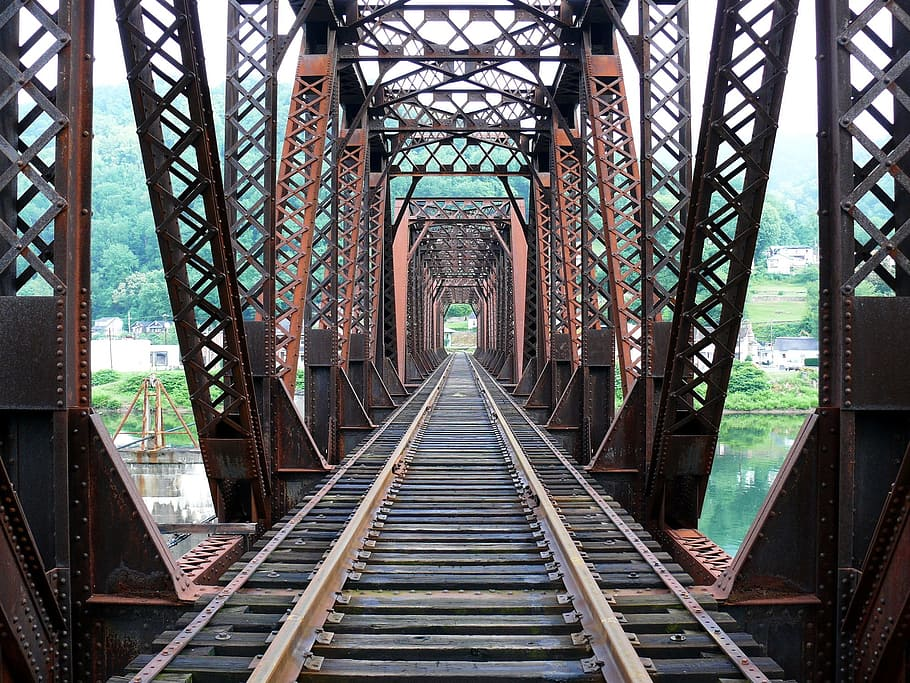
\includegraphics[width=0.45\columnwidth]{Chap05LU/railroad-bridge-tracks-rails-trusses.jpg}}%
\hspace{5pt}%
\subfloat[]{%
    \label{fig:Roof}%
	\centering
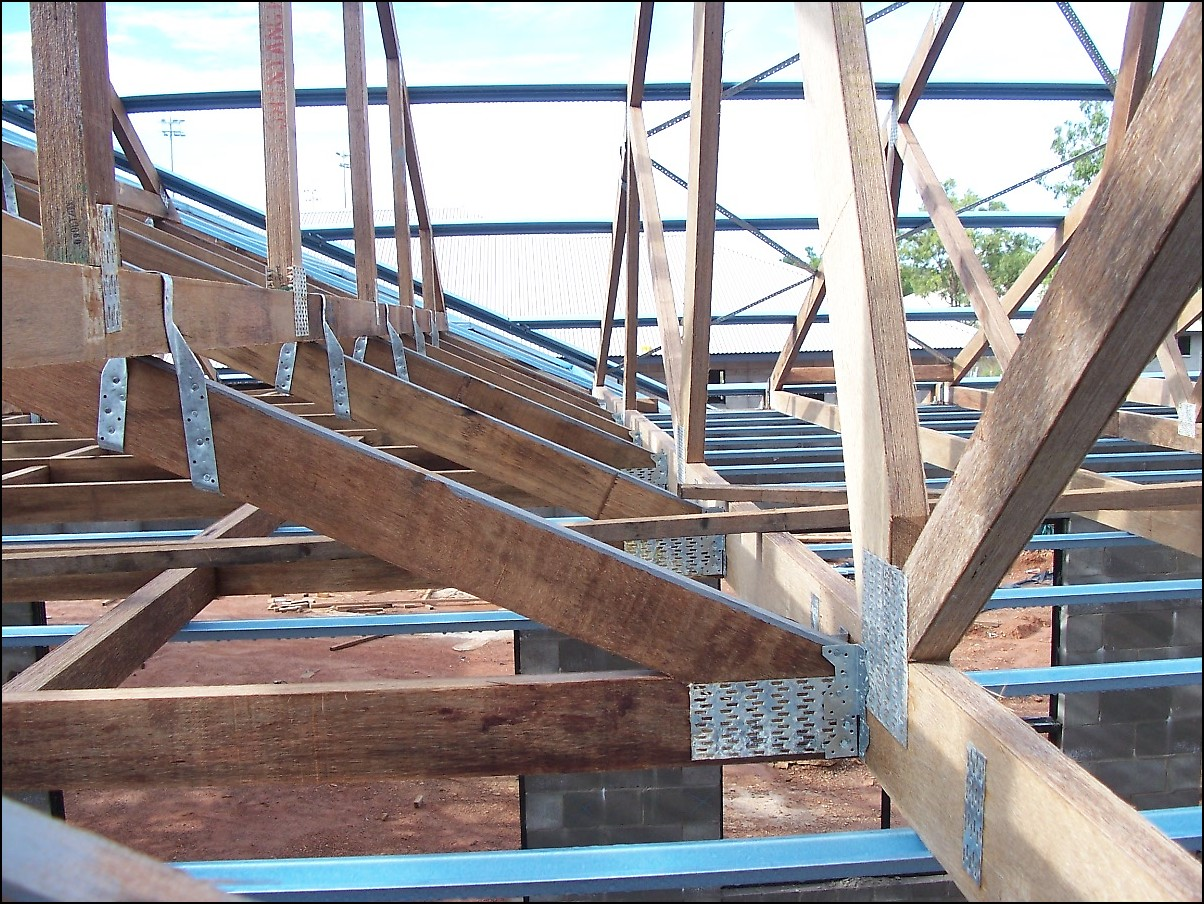
\includegraphics[width=0.45\columnwidth]{Chap05LU/Truss-roof.jpg}}%
    \caption[]{Trusses are ubiquitous in construction. Here we show two uses in bridges and roofs. The techniques used to analyze the forces in each member of a truss are taught in ME 211. They result in a large set of linear equations. We'll use a bridge to exemplify the main ideas. You can learn more at \url{https://www.youtube.com/watch?v=Hn_iozUo9m4}.}
    \label{fig:TrussStructures}
\end{figure}

\begin{figure}[hbt!]%
\centering
\subfloat[]{%
    \label{fig:SimpleBridge}%
	\centering
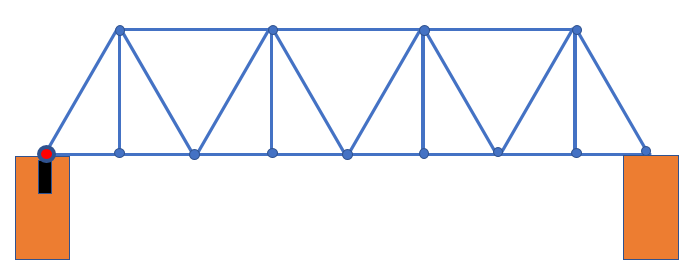
\includegraphics[width=0.75\columnwidth]{Chap05LU/TrussBridgeJWG.png}}%
\hspace{5pt}%
\subfloat[]{%
    \label{fig:bridgeJoingLabels}%
	\centering
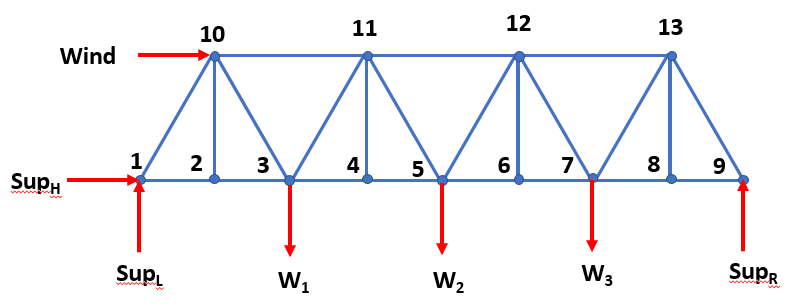
\includegraphics[width=0.65\columnwidth]{Chap05LU/TrussBridgeJWGExternalForces.png}}%
\hspace{5pt}%
\subfloat[]{%
    \label{fig:FreeBodyDiagram}%
	\centering
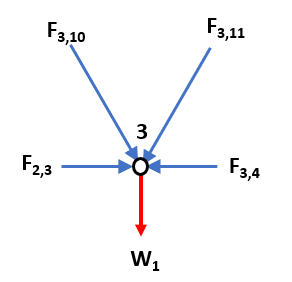
\includegraphics[width=0.25\columnwidth]{Chap05LU/TrussBridgeJWGForceLabelsConvention.png}}%
    \caption[]{A planar truss bridge over an open span, say a road or body of water. As shown in (a), the bridge is pinned on the left and ``floating'' on the right. In (b), the joints of the truss structure have been labeled along with some of the forces, such as the horizontal and vertical forces at the left support point, the vertical force at the right support point, wind loading on the structure, and a simplified representation of the structure's weight pulling down on it. A free body diagram for joint 3 is shown in (c), where it is assumed \textit{arbitrarily} that each member is in compression. If a member is in \textit{tension} instead of compression, the force will be a negative number. To build the linear model for the truss structure, force balances must be computed at each joint in the horizontal and vertical directions. Because there are 13 joints, the model will have 26 variables in it. The real-life structures in Fig.~\ref{fig:TrussStructures} would have several hundreds of variables.}
    \label{fig:TrussBridgeCartoons}
\end{figure}

Figure~\ref{fig:TrussStructures} shows two truss structures, one for a railroad bridge and the other for a roof in a house or small office building. We'll analyze the simpler planar truss bridge in Fig.~\ref{fig:TrussBridgeCartoons},  which has joints labeled 1 to 13. In case you are interested, the basic method used to develop a mathematical model of the structure is taught in ME 211 Introduction to Dynamics and Vibrations. At each joint, a free body diagram is constructed as shown in Fig.~\ref{fig:TrussBridgeCartoons}-(c), where it has been arbitrarily assumed that all of the members in the truss are in \textit{compression}, and thus the forces transmitted by them are directed \textit{into the joint}. With this convention, when we eventually solve for the indicated forces, any member that is in \textit{tension will have a negative force associated to it}. \\

The angled members in the diagram form an angle of $\frac{\pi}{3}$, or $60^\circ$, with respect to the horizontal axis. The force balance at joint 3 yields two equations,
\begin{equation}
    \begin{aligned}
    F_{2,3}-F_{3,4}+\cos(\pi/3) F_{3,10}-\cos(\pi/3) F_{3,11} &=0.0~~~~ \textbf{horizontal components}\\
  -F_{w1}-\sin(\pi/3) F_{3,10}-\sin(\pi/3) F_{3,11}  & = 0.0~~~~ \textbf{vertical components,}
    \end{aligned}
\end{equation}
the first for the horizontal components of the forces and the second for the vertical components of the forces. A similar process at joint 10 yields
\begin{equation}
    \begin{aligned}
    F_{\rm wind}-F_{10,11}+\cos(\pi/3) F_{1,10}-\cos(\pi/3) F_{3,10} &=0.0~~~~ \textbf{horizontal components}\\
  F_{2,10}+\sin(\pi/3) F_{1,10}+\sin(\pi/3) F_{3,10}  & = 0.0~~~~ \textbf{vertical components.}
    \end{aligned}
\end{equation}
Repeating this for each of the 13 joints yields a total of 26 equations for the 26 unknown forces. \textbf{The resulting linear system of equations $Ax=b$ has an $A$ matrix that is $26 \times 26$, which means it has 676 entries. \textcolor{red}{As you can imagine, building the matrix by hand would be very tedious! What to do about it? Write some code! The Julia code below is a bit advanced for where we are right now in ROB 101. It is included for the sole purpose of illustrating that programming can be used to build models as well as to solve equations.}}\\

The Julia code contains each of the 26 force balance equations, then from the force balance equations it creates the model $Ax=b$, and finally it solves for $x$ by LU factorization with row permutations. You are not expected to work through and understand the code. Copying it into a \texttt{jupyter notebook} and playing with it may be fun. You can check that $\det(A)\approx 1.46$. 

\begin{lstlisting}[language=Julia,style=mystyle]
using LinearAlgebra

function Model(x,u)
#  Units are kilo Newtons, or the force required to support 220 pounds
#  Bridge model variables
    # External forces
    Fw1=u[1];Fw2=u[2];Fw3=u[3];Fwind=u[4]
    # Internal Forces, where "c" stands for "comma"
    F1c2=x[1]
    F1c10=x[2]
    F2c3=x[3]
    F2c10=x[4]
    F3c4=x[5]
    F3c10=x[6]
    F3c11=x[7]
    F4c5=x[8]
    F4c11=x[9]
    F5c6=x[10]
    F5c11=x[11]
    F5c12=x[12]
    F6c7=x[13]
    F6c12=x[14]
    F7c8=x[15]
    F7c12=x[16]
    F7c13=x[17]
    F8c9=x[18]
    F8c13=x[19]
    F9c13=x[20]
    F10c11=x[21]
    F11c12=x[22]
    F12c13=x[23]
    FhorizLeft=x[24]
    FvertLeft=x[25]
    FvertRight=x[26]
#Bridge force balance equations
    # Note cos(pi/3)=0.5 and sin(pi/3)=sqrt(3)/2
    #joint 1, x component first then y 
    Eq1x=FhorizLeft-F1c2-F1c10*cos(pi/3)
    Eq1y=FvertLeft-F1c10*sin(pi/3)
    #joint 2, x component first then y 
    Eq2x=F1c2-F2c3
    Eq2y=F2c10
    #joint 3, x component first then y 
    Eq3x=F2c3-F3c4+cos(pi/3)*F3c10-cos(pi/3)*F3c11
    Eq3y=-Fw1-sin(pi/3)*F3c10-sin(pi/3)*F3c11
    #joint 4, x component first then y 
    Eq4x=F3c4-F4c5
    Eq4y=-F4c11
    #joint 5, x component first then y 
    Eq5x=F4c5-F5c6+cos(pi/3)*F5c11-cos(pi/3)*F5c12
    Eq5y=-Fw2-sin(pi/3)*F5c11-sin(pi/3)*F5c12
    #joint 6, x component first then y 
    Eq6x=F5c6-F6c7
    Eq6y=-F6c12
    #joint 7, x component first then y 
    Eq7x=F6c7-F7c8+cos(pi/3)*F7c12-cos(pi/3)*F7c13
    Eq7y=-Fw3-sin(pi/3)*F7c12-sin(pi/3)*F7c13
    #joint 8, x component first then y 
    Eq8x=F7c8-F8c9
    Eq8y=-F8c13
    #joint 9, x component first then y 
    Eq9x=F8c9+F9c13*cos(pi/3)
    Eq9y=FvertRight-F9c13*sin(pi/3)
    #joint 10, x component first then y 
    Eq10x=Fwind-F10c11+cos(pi/3)*F1c10-cos(pi/3)*F3c10
    Eq10y=F2c10+sin(pi/3)*F1c10+sin(pi/3)*F3c10
    #joint 11, x component first then y 
    Eq11x=F10c11-F11c12+cos(pi/3)*F3c11-cos(pi/3)*F5c11
    Eq11y=F4c11+sin(pi/3)*F3c11+sin(pi/3)*F5c11
    #joint 12, x component first then y 
    Eq12x=F11c12-F12c13+cos(pi/3)*F5c12-cos(pi/3)*F7c12
    Eq12y=F6c12+sin(pi/3)*F5c12+sin(pi/3)*F7c12
    #joint 13, x component first then y 
    Eq13x=F12c13+cos(pi/3)*F7c13-cos(pi/3)*F9c13
    Eq13y=F8c13+sin(pi/3)*F7c13+sin(pi/3)*F9c13
    # Place all of the equations in a vector
    y=[Eq1x;Eq1y;Eq2x;Eq2y;Eq3x;Eq3y;Eq4x;Eq4y;Eq5x;Eq5y;Eq6x;Eq6y;Eq7x;Eq7y;Eq8x;Eq8y;Eq9x;Eq9y;Eq10x;Eq10y;Eq11x;Eq11y;Eq12x;Eq12y;Eq13x;Eq13y]
return y
end
# Query the equations to build the model in the form Ax=b
n=26
m=4
A=Array{Float64,2}(undef, n, 0)
Id=zeros(n,n)+I
#
for k =1:n
    ek=Id[:,k]
    ak=Model(ek,zeros(m,1))
    A=[A ak]
#    @show ak
end
@show det(A)
@show size(A)
Fw1=2000  #kilo Newtons
Fw2=3000
Fw3=2000
Fwind=500.
u=[Fw1;Fw2;Fw3;Fwind]
b=-Model(zeros(n,1),u)
# Solve the equations
# Uncomment the next line to see if A can be factored without permutations
#F=lu(A,Val(false)) 
F=lu(A) 
L=F.L
U=F.U
P=F.P
# the functions forwardsub and backwardsub are NOT given. You learned how to
# write them in previous chapters.
y=forwardsub(L, P*b)
x=backwardsub(U, y)
\end{lstlisting}
\vspace*{.2cm}
Here is the solution to $Ax=b$,
\begin{equation}
x=\left[
\begin{array}{r}
-2458.2 \\
3916.5 \\
-2458.2 \\
\RED 0.0 \\
-5220.0 \\
-3916.5 \\
1607.1 \\
-5220.0 \\
\RED 0.0 \\
-5095.0 \\
-1607.1 \\
-1857.1 \\
-5095.0 \\
\RED 0.0 \\
-2083.2 \\
1857.1 \\
-4166.5 \\
-2083.2 \\
\RED 0.0 \\
4166.5 \\
4416.5 \\
6023.5 \\
4166.5 \\
-500.0 \\
3391.7 \\
3608.3 \\
\end{array}
\right]_{26 \times 1}.
\end{equation}
The variable names are in the code. We see that there are four ``zero force members'' highlighted in red, the beams between joints 2 and 10, 4 and 11, 6 and 12, and 8 and 13. While they are not load bearing elements in the nominal structure, they provide important rigidity to the structure and they serve as safety elements in case one of the angled beams should fail. Finally, from the minus signs, we see that under the given loading conditions, more than half of the beams are in tension. We emphasize that this does not invalidate our analysis as tension vs compression is merely a direction convention, just like us assuming that forces that point up or to the right are acting in a positive direction. 
\newpage

\section{(Optional Read): An Algorithm for Rectangular LU Factorization with Row Permutations}

In section 5.6, you were given an algorithm which generates the LU factorization of square matrices. However, it turns out that we do not need much modification to also handle rectangular matrices!
 
 \begin{tcolorbox}[sharp corners, colback=green!30, colframe=green!80!blue, title=\textbf{\Large LU Factorization of Matrices}]
 \begin{algorithm}[H]
\SetAlgoLined
\KwResult{For M an $a \times b$ rectangular matrix, with $a\ge2$ and $b\ge2$, find $L$, $U$, and $P$ such that $PM=LU$}
\mbox{} \\
 \textbf{initialization:}\\
 {\rm Temp}=copy(M); \\
 n = min(a, b)
L = Array\{Float64,2\}(undef, a, 0)  ~~~\# L=[] Empty matrix\\
U = Array\{Float64,2\}(undef, 0, b)  ~~~\# U=[] Empty matrix\\
 P= I$_a$ \# $a \times a$ identity matrix\\
 eps= 1e-16 \# estimate of machine epsilon \\
 Kappa = 100  \#How small is too small for you?\\
  \textbf{end of initialization:}\\
\mbox{}  \\
% \textbf{for } {k=1:n}\\
\For{k=1:n}
 {
    C=Temp[:,k]; \# k-th column\\
    R={\rm Temp}[k,:]'; \# k-th row\\
    \eIf{ max(abs(C)) <= Kappa*eps \# (check for C all zeros) }
  { 
      C=0*C \# Set tiny values to zero\\
      C[k]=1.0 \\
    {\rm Temp}={\rm Temp}-C*R; \\
     L=[L,C]  \# Build the lower-triangular matrix by columns\\
    U=[U;R] \# Build the upper-triangular matrix by rows
   }
   {
   \# We know C has at least one non-zero quantity \\ 
    \# We'll bring its largest entry to the top; \\
    \# while this is overkill, it helps with numerical aspects of the algorithm \\
    \# Bringing biggest to top will always avoid divide by zero \\
    \# It's enough to bring ANY non-zero value to the top \\
    \# \\
   nrow=argmax(abs(C)) \# find the index where C is ``biggest'' \\
   P[[k,nrow],:]=P[[nrow,k],:] \# permute (i.e., swap) rows of P  \\
  {\rm Temp}[[k,nrow],:]={\rm Temp}[[nrow,k],:] \# do same for {\rm Temp}\\
   \# if L is non-empty, also swap its rows \\
   \If{k > 1}{ L[[k,nrow],:]=L[[nrow,k],:] } {}
    C=Temp[:,k]; \# k-th column\\
    pivot = C[k]\\
    C=C/pivot \#divide all elements of C by the pivot \\
    R={\rm Temp}[k:k,:] \# k-th row\\
     {\rm Temp}={\rm Temp}-C*R; \\
     L=[L C]  \# Build the lower-triangular matrix by columns\\
    U=[U;R] \# Build the upper-triangular matrix by rows \\
  }
}
\textbf{return L, U, P}
\end{algorithm}
\end{tcolorbox}
   
\newpage

\section{Looking Ahead}

Once you have programmed in Julia 
\begin{enumerate}
\renewcommand{\labelenumi}{(\alph{enumi})}
\setlength{\itemsep}{.2cm}
    \item  algorithms for forward and back substitution (methods for solving triangular systems of equations), and 
    \item  the LU Factorization Algorithm, 
\end{enumerate}
you will be well placed for solving systems of linear equations of very large dimension. In the next chapter, we will fill in some of the more standard results that students learn in linear algebra, where the focus is on solving ``drill problems'' and not ``real engineering problems''.  In your later courses, most instructors will simply assume you know the more standard material and that you have no clue about the more nuanced approach to problem solving that we have developed in ROB 101. We'll do our best to throw in some cool computational aspects as we go.\\

